\documentclass{article}
\usepackage[utf8]{inputenc} % Поддержка UTF-8
\usepackage[T2A]{fontenc}   % Кодировка T2A для кириллицы
\usepackage[russian]{babel} % Поддержка русского языка
\usepackage{graphicx}       % Для вставки изображений
\usepackage{listings}       % Для блоков кода
\usepackage{listingsutf8}   % Поддержка UTF-8 в listings
\usepackage{xcolor}         % Цвета для кода
\usepackage{geometry}       % Настройка полей
\usepackage{float}          % Для управления плавающими объектами
\usepackage{amsmath}
\usepackage{amsfonts}
\usepackage{amssymb}

\geometry{top=2.2cm, bottom=2.2cm, left=2.2cm, right=2.3cm}

\lstset{
	language=Java,
	basicstyle=\ttfamily\footnotesize,
	keywordstyle=\color{blue},
	stringstyle=\color{red},
	commentstyle=\color{green},
	numbers=left,
	numberstyle=\tiny\color{gray},
	numbersep=5pt,
	backgroundcolor=\color{white}
}

\begin{document}
	\newcommand{\university}{Министерство науки и высшего образования Российской Федерации
	
	Федеральное государственное автономное образовательное учреждение высшего образования
	
	«Национальный исследовательский университет ИТМО»}
\newcommand{\mfaculty}{Мегафакультет компьютерных технологий и управления}
\newcommand{\faculty}{Факультет Программной инженерии и компьютерной техники}
\newcommand{\city}{Санкт-Петербург}
\newcommand{\num}{№4}
\newcommand{\docname}{Лабораторная работа}
\newcommand{\subject}{Основы программной инженерии}
\newcommand{\tutorname}{Миху Вадим Дмитриевич}
\newcommand{\studentname}{Здор Матвей Максимович}
\newcommand{\group}{P3224}
\newcommand{\variant}{2329}
	\include{titlepage}
	\newpage
	\tableofcontents
	\newpage
	
	\section{Задание}
	\begin{figure}[H]
		\centering
		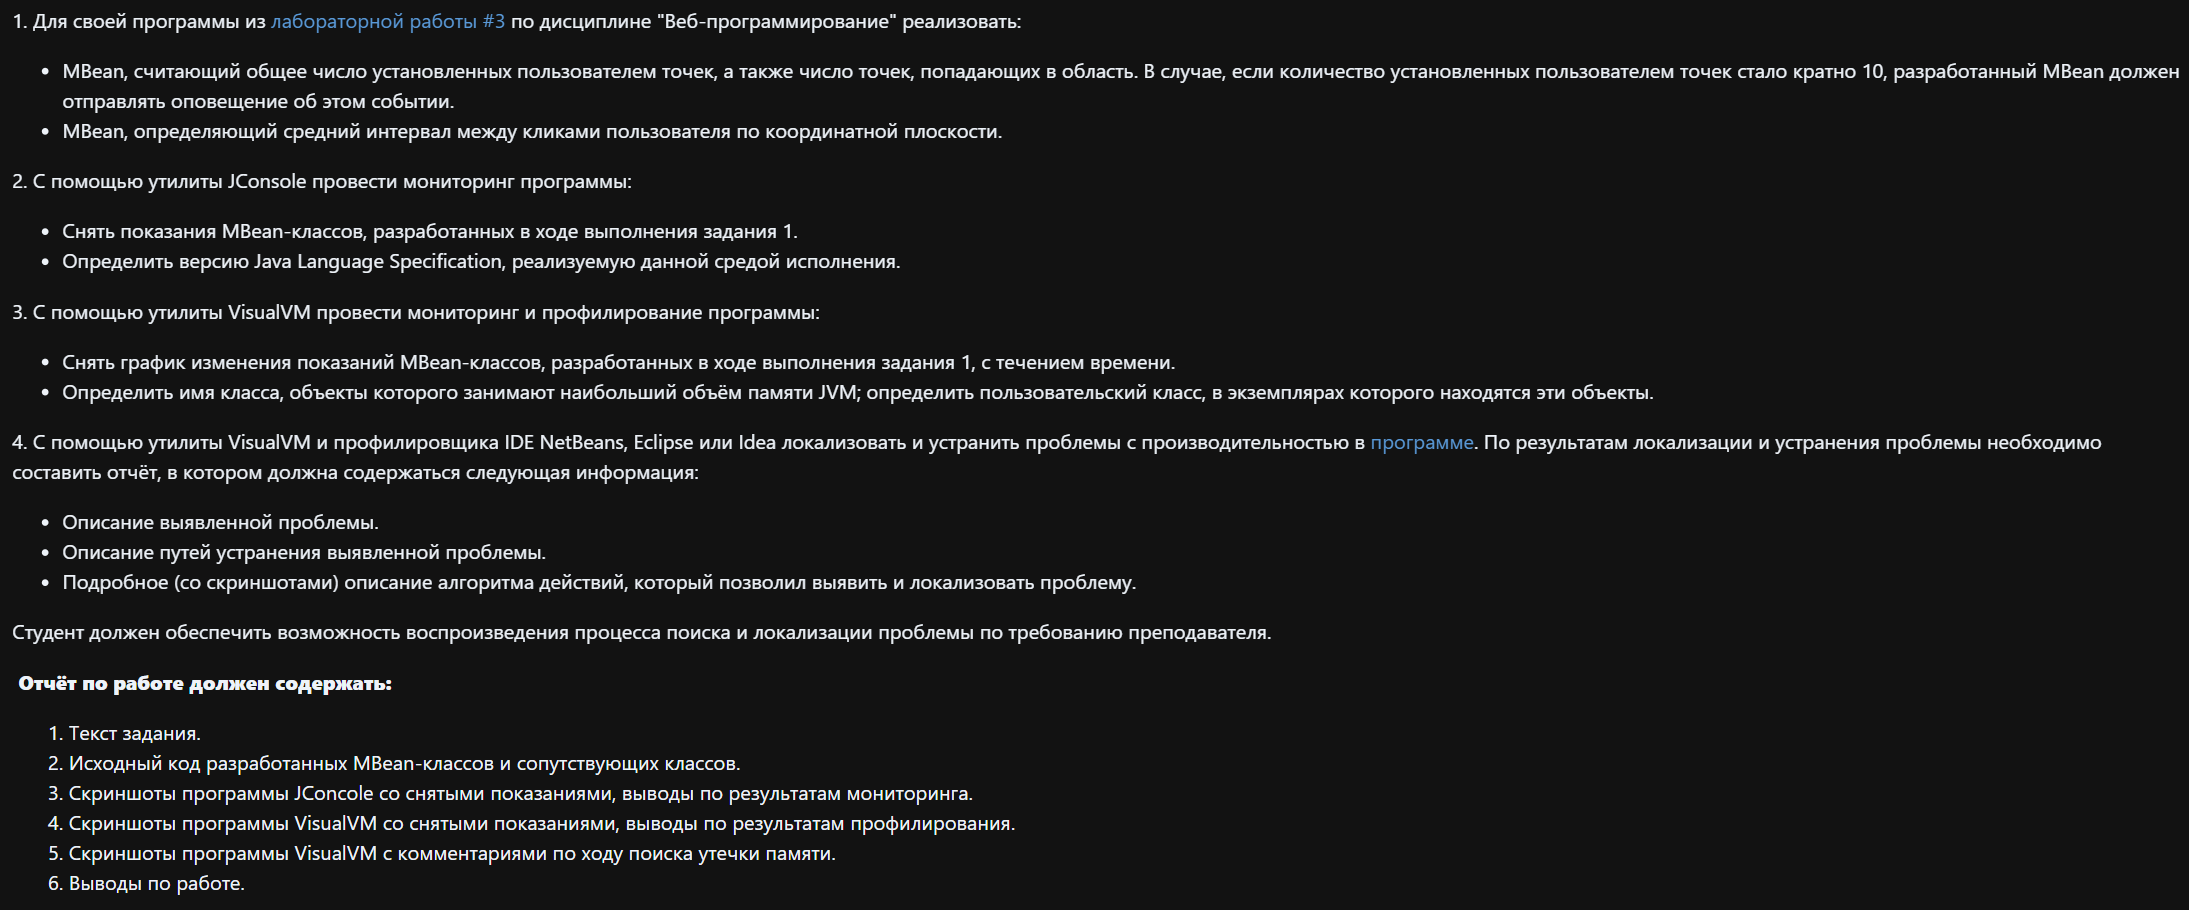
\includegraphics[width=1\linewidth]{images/task}
		\caption{Текст задания лабораторной работы}
		\label{fig:task}
	\end{figure}
	
	\newpage
	
	\section{Реализация MBean’ов}
	
	\subsection{MBean для подсчёта общего числа установленных точек и числа точек вне области с отправкой оповещения при выходе за границы}
	Класс реализует MBean интерфейс для учёта всех точек и точек, вышедших за границы области, с генерацией JMX-уведомления при превышении порогового значения.
	\begin{lstlisting}[language=Java, caption=PointsCounterMBean.java]
package ru.itmo.web.lab3.beans;

import ru.itmo.web.lab3.model.Point;

public interface PointsCounterMBean {
	void proceedPoint(Point point);
	int getPointsCounter();
	int getHitsCounter();
	void resetCounters();
}

	\end{lstlisting}
	\begin{lstlisting}[language=Java, caption=PointsCounter.java]
package ru.itmo.web.lab3.beans;

import jakarta.enterprise.context.ApplicationScoped;
import lombok.Setter;
import ru.itmo.web.lab3.model.Point;

import javax.management.Notification;
import javax.management.NotificationBroadcasterSupport;
import javax.management.ObjectName;
import java.io.Serializable;

@ApplicationScoped
public class PointsCounter extends NotificationBroadcasterSupport
implements PointsCounterMBean, Serializable {
	private int pointsCounter = 0;
	private int hitsCounter = 0;
	private long notificationSequence = 0;
	@Setter
	private ObjectName objectName;
	@Override
	public void proceedPoint(Point point) {
		if(point.isHit()) {
			hitsCounter++;
		}
		pointsCounter++;
		checkTenPoints();
	}
	
	@Override
	public int getPointsCounter() {
		return pointsCounter;
	}
	
	@Override
	public int getHitsCounter() {
		return hitsCounter;
	}
	
	@Override
	public void resetCounters() {
		pointsCounter = 0;
		hitsCounter = 0;
	}
	
	void checkTenPoints() {
		if(pointsCounter % 10 == 0) {
			Notification notification = new Notification(
			"PointsCounter Notification",
			this,
			notificationSequence++,
			System.currentTimeMillis(),
			"Reached " + pointsCounter + " points");
			sendNotification(notification);
		}
	}
}

	\end{lstlisting}
	
	\newpage
	
	\subsection{MBean для определения среднего интервала между кликами пользователя}
	Класс предназначен для измерения и усреднения времени между последовательными событиями клика.
	\begin{lstlisting}[language=Java, caption=AverageClickTimeMBean.java]
package ru.itmo.web.lab3.beans;

import ru.itmo.web.lab3.model.Point;

public interface AverageClickTimeMBean {
	long getAverageClickTime();
	void reset();
	void proceedPoint(Point point);
}
	\end{lstlisting}
	\begin{lstlisting}[language=Java, caption=AverageClickTime.java]
package ru.itmo.web.lab3.beans;

import jakarta.enterprise.context.ApplicationScoped;
import lombok.Setter;
import lombok.extern.log4j.Log4j2;
import ru.itmo.web.lab3.model.Point;

import javax.management.MBeanServer;
import javax.management.ObjectName;
import java.lang.management.ManagementFactory;
import java.time.Duration;
import java.time.LocalDateTime;

@ApplicationScoped
@Log4j2
public class AverageClickTime implements AverageClickTimeMBean {
	@Setter
	private ObjectName objectName;
	@Setter
	private ObjectName pointsCounterObjectName;
	private LocalDateTime firstClickTime;
	private LocalDateTime lastClickTime;
	private int pointsCount;
	private final MBeanServer mBeanServer;
	private long averageClickTime;
	
	public AverageClickTime() {
		this.mBeanServer = ManagementFactory.getPlatformMBeanServer();
		this.firstClickTime = null;
		this.lastClickTime = null;
		this.pointsCount = 0;
	}
	
	@Override
	public long getAverageClickTime() {
		return averageClickTime;
	}
	
	@Override
	public void proceedPoint(Point point) {
		if (point == null || point.getCheckTime() == null) {
			return;
		}
		
		if (firstClickTime == null) {
			firstClickTime = point.getCheckTime();
		}
		
		lastClickTime = point.getCheckTime();
		
		try {
			pointsCount = (Integer) mBeanServer.getAttribute(pointsCounterObjectName, "PointsCounter");
			log.info("Number of points in first click: {}", pointsCount);
		} catch (Exception e) {
			log.error("Failed to get PointsCounter", e);
			pointsCount = 0;
		}
		
		if (firstClickTime == null || lastClickTime == null || pointsCount <= 1) {
			averageClickTime = -1;
			log.info("Average click time is incorrect");
			log.info("firstClickTime: {}", firstClickTime);
			log.info("lastClickTime: {}", lastClickTime);
			log.info("pointsCount: {}", pointsCount);
			return;
		}
		
		try {
			long durationMillis = Duration.between(firstClickTime, lastClickTime).toMillis();
			averageClickTime =  durationMillis / (pointsCount - 1);
			log.info("New average click time: {}", averageClickTime);
		} catch (Exception e) {
			e.printStackTrace();
			averageClickTime = -500;
		}
	}
	
	@Override
	public void reset() {
		firstClickTime = null;
		lastClickTime = null;
		pointsCount = 0;
	}
}
	\end{lstlisting}
	
	\section{Мониторинг с помощью JConsole}
	
	\begin{figure}[H]
		\centering
		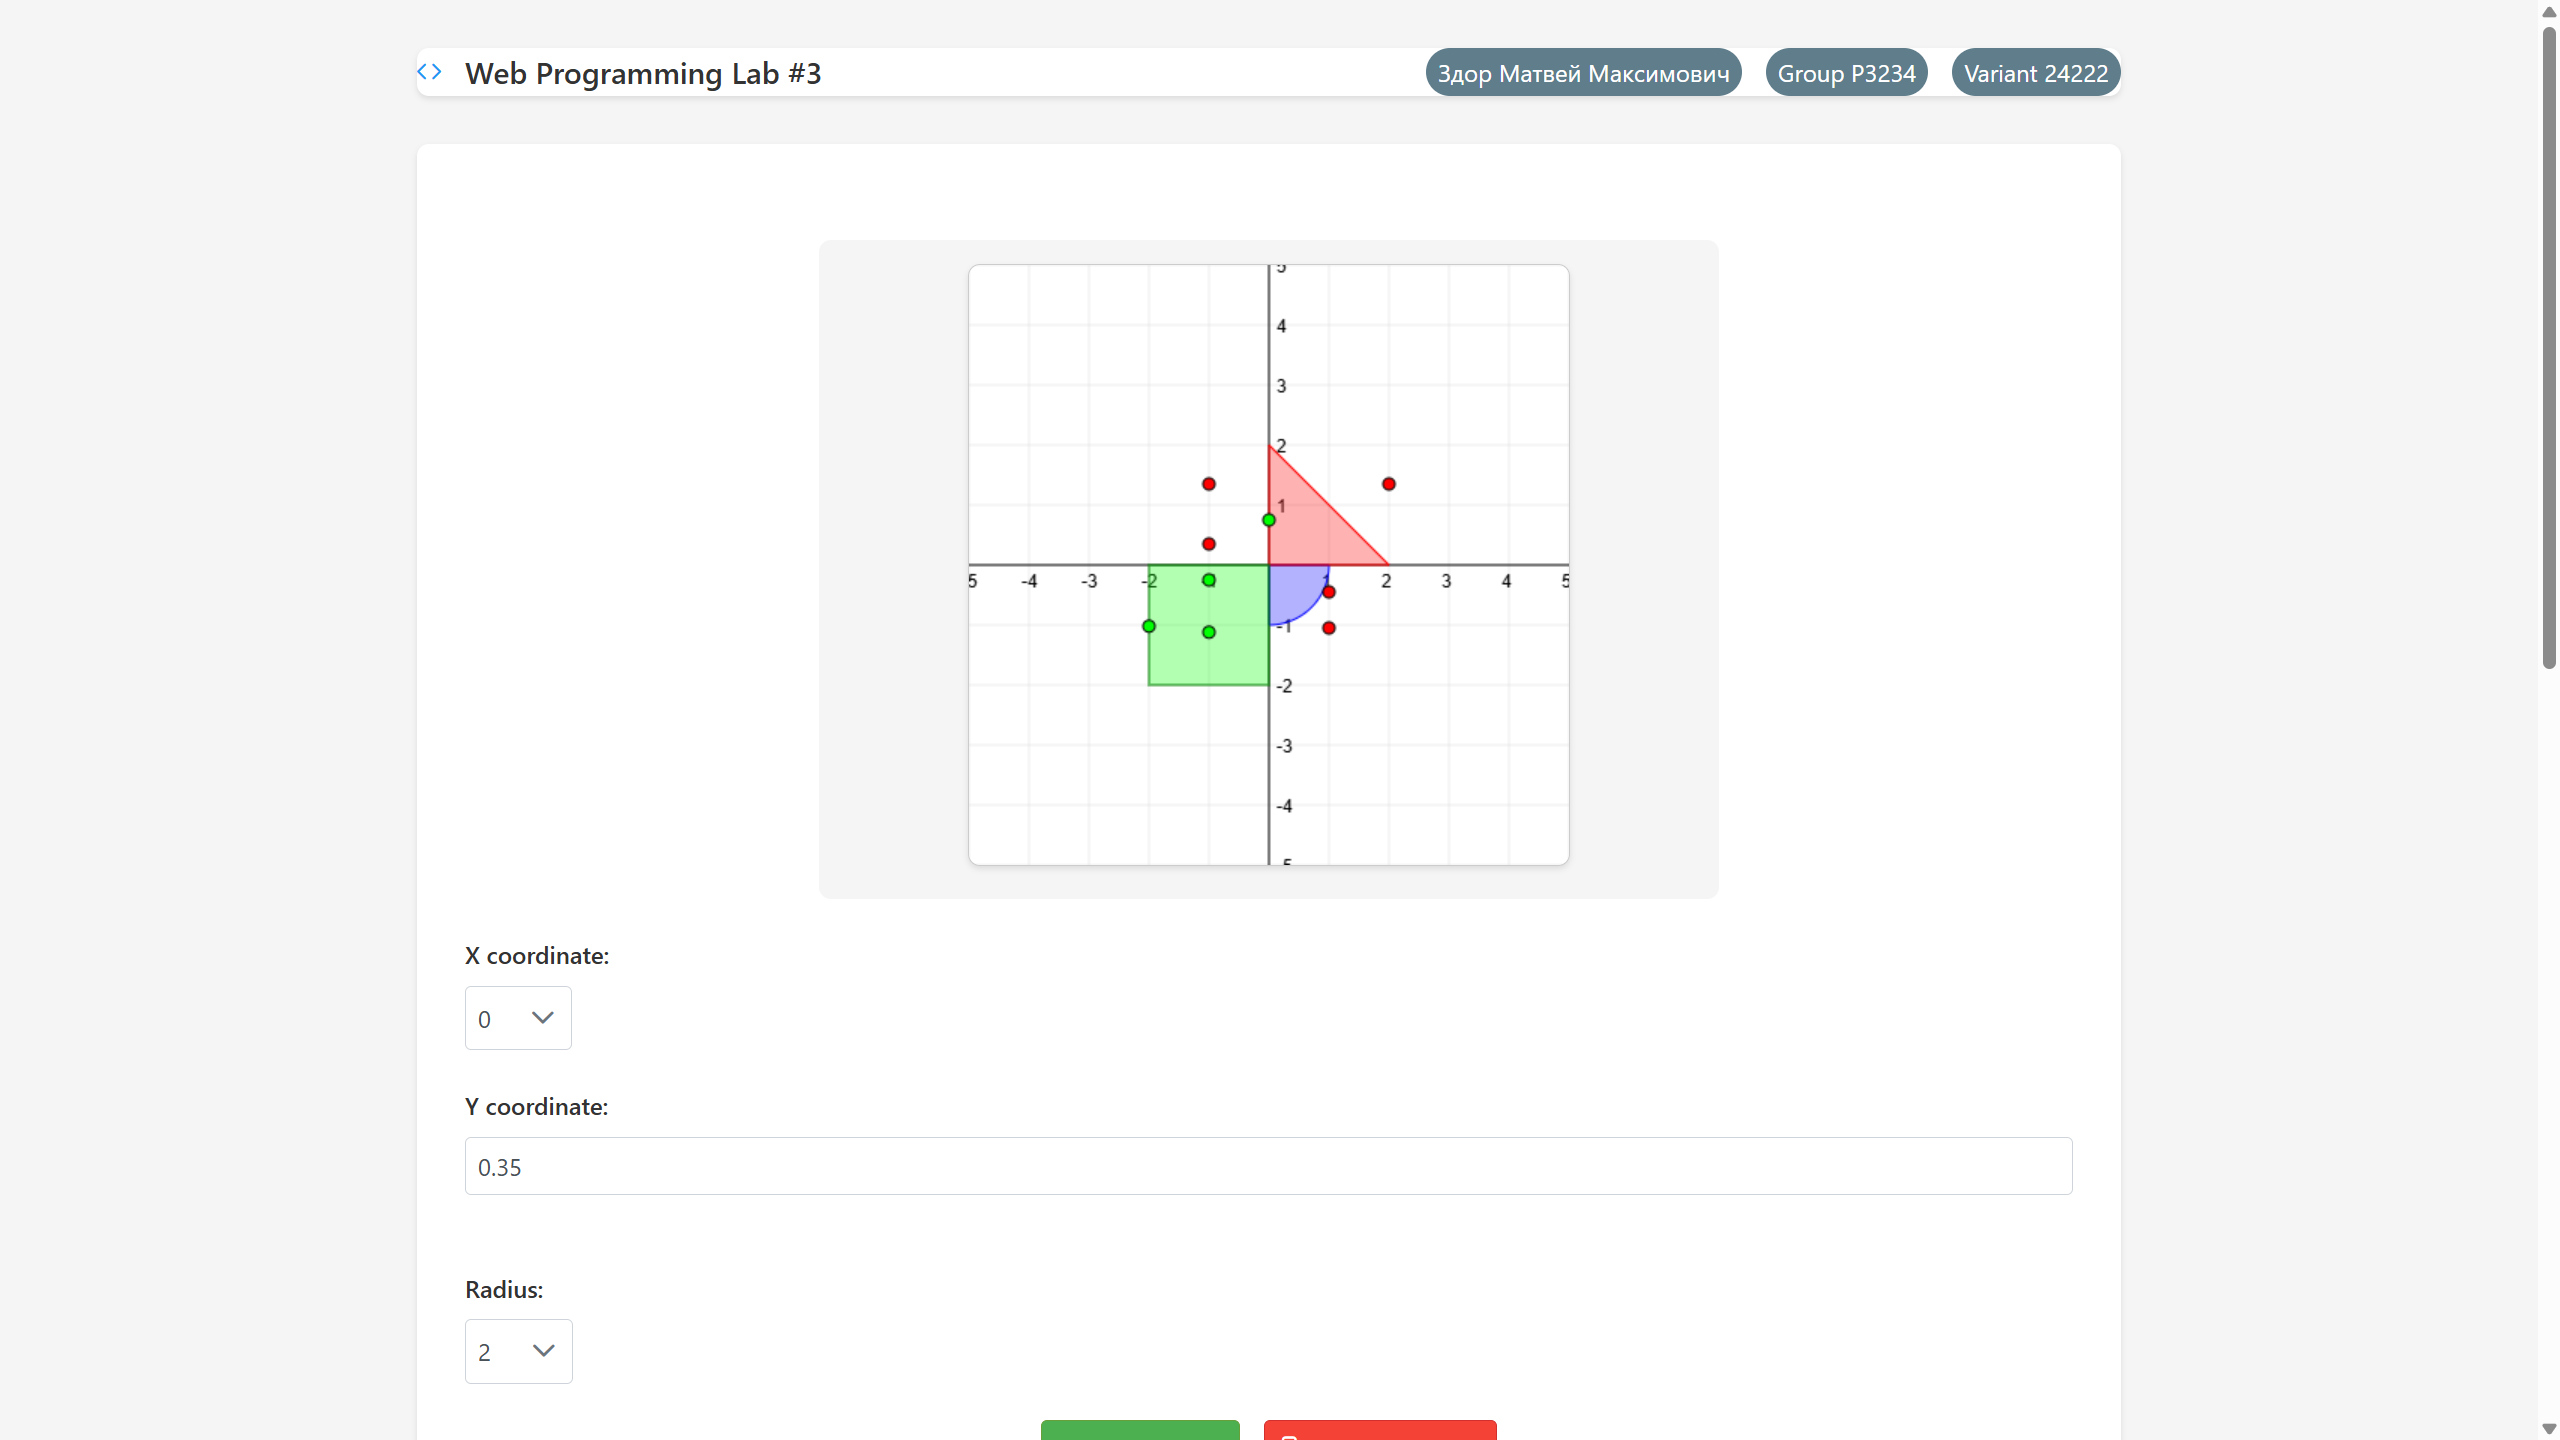
\includegraphics[width=1\linewidth]{jconsole/web_page}
		\caption{Интерфейс веб-приложения с координатной плоскостью для установки точек}
		\label{fig:webpage}
	\end{figure}
	
	\subsection{Снятие показаний MBean-классов}
	\begin{figure}[H]
		\centering
		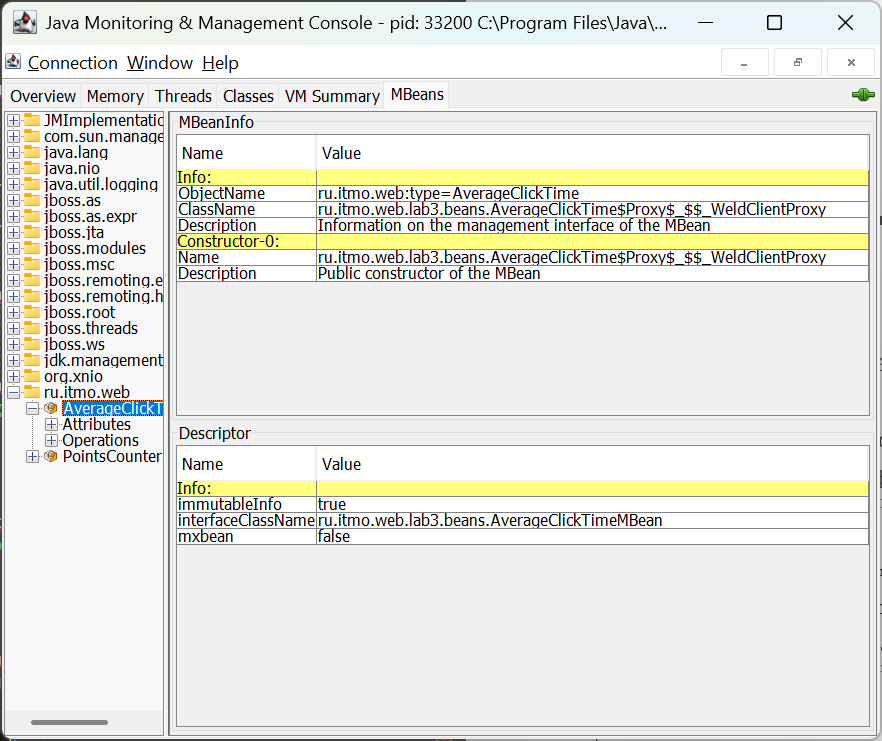
\includegraphics[width=1\linewidth]{jconsole/average_time_bean}
		\caption{Просмотр MBean AverageClickTime в JConsole}
		\label{fig:averagetimebean}
	\end{figure}
	\begin{figure}[H]
		\centering
		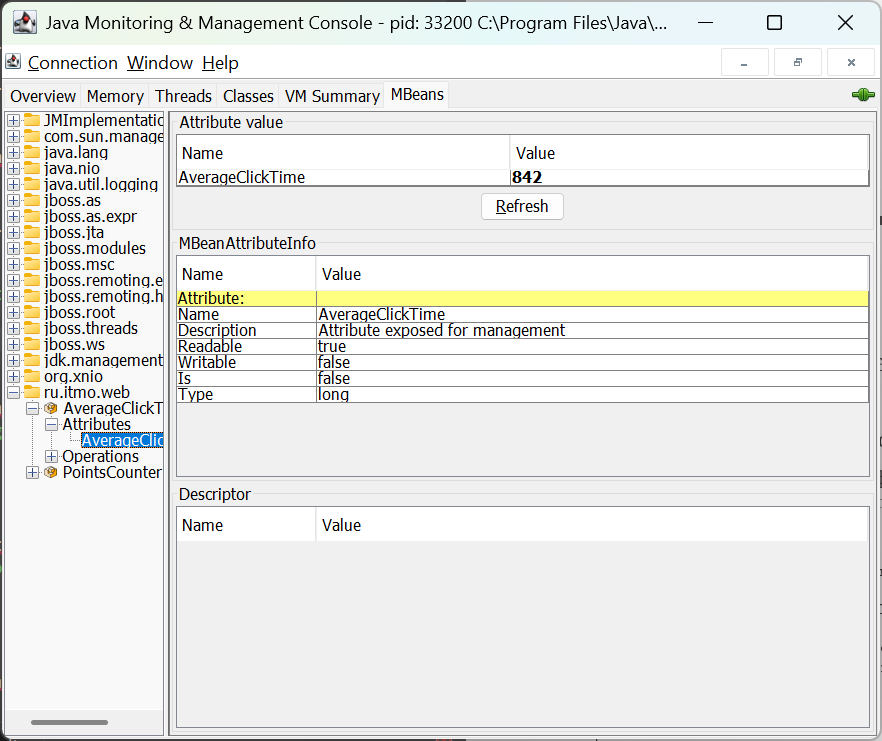
\includegraphics[width=1\linewidth]{jconsole/average_time_bean_atributes}
		\caption{Атрибуты MBean AverageClickTime, отображающие среднее время между кликами}
		\label{fig:averagetimebeanatributes}
	\end{figure}
	
	\begin{figure}[H]
		\centering
		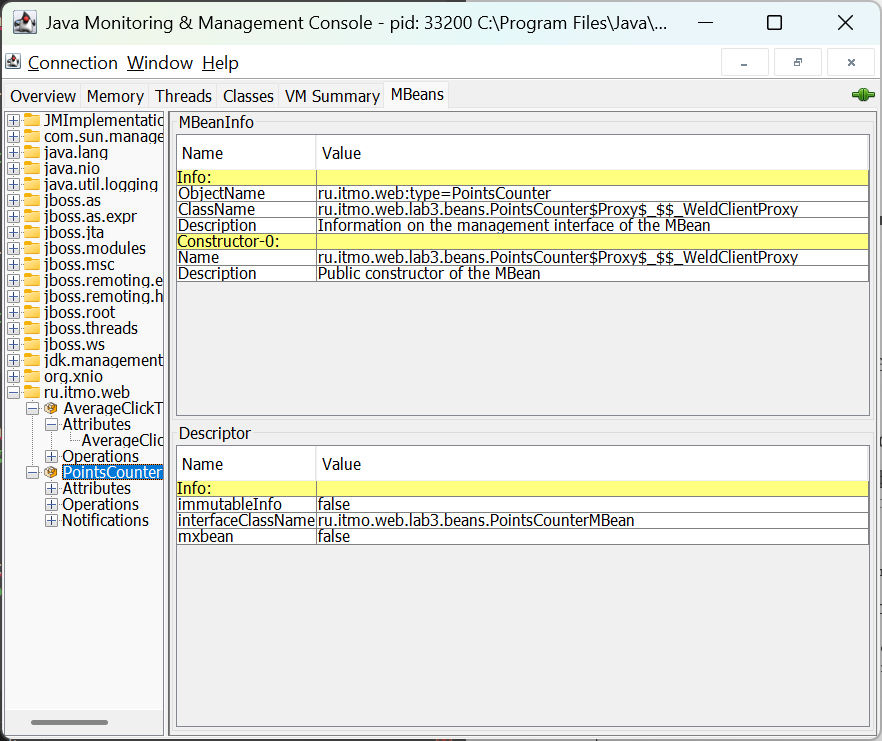
\includegraphics[width=1\linewidth]{jconsole/points_counter}
		\caption{Просмотр MBean PointsCounter в JConsole}
		\label{fig:pointscounter}
	\end{figure}
	\begin{figure}[H]
		\centering
		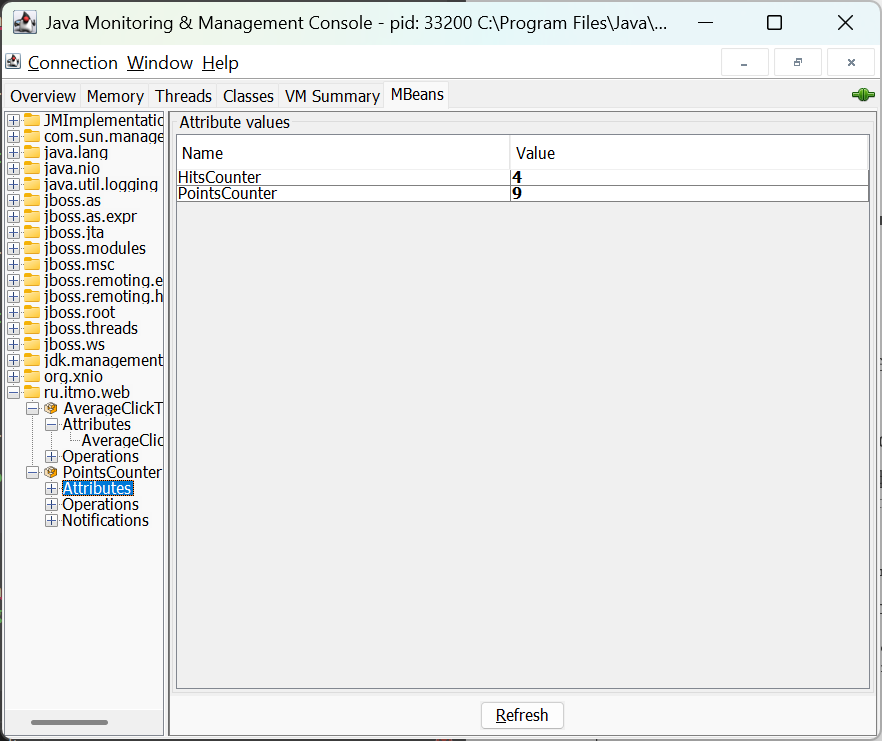
\includegraphics[width=1\linewidth]{jconsole/points_counter_atributes}
		\caption{Атрибуты MBean PointsCounter: общее число точек и число попаданий}
		\label{fig:pointscounteratributes}
	\end{figure}
	
	\begin{figure}[H]
		\centering
		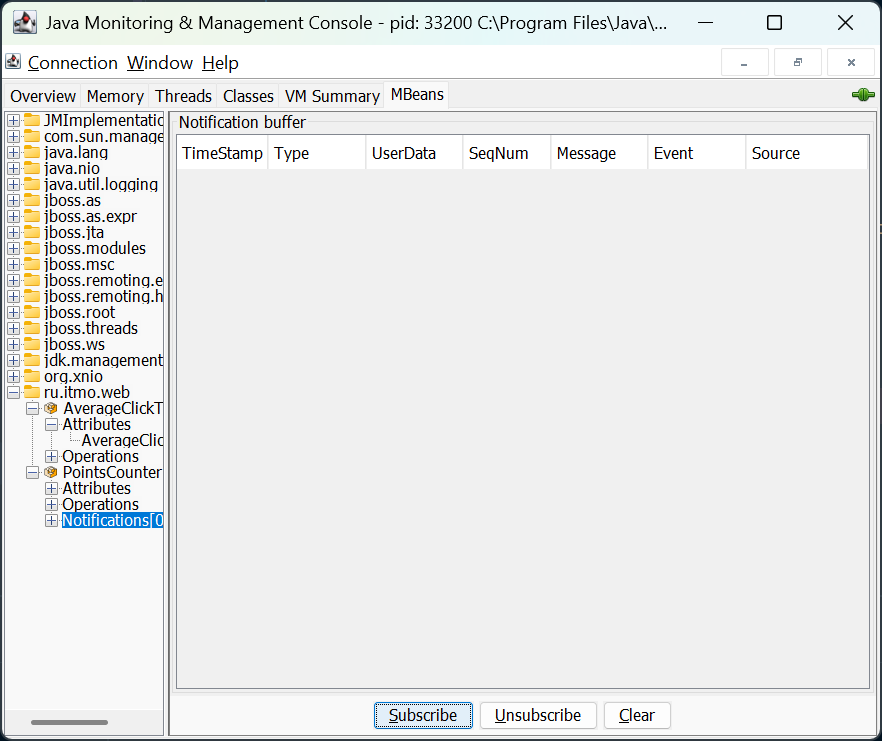
\includegraphics[width=1\linewidth]{jconsole/subscription}
		\caption{Подписка на уведомления от PointsCounter в JConsole}
		\label{fig:subscription}
	\end{figure}
	\begin{figure}[H]
		\centering
		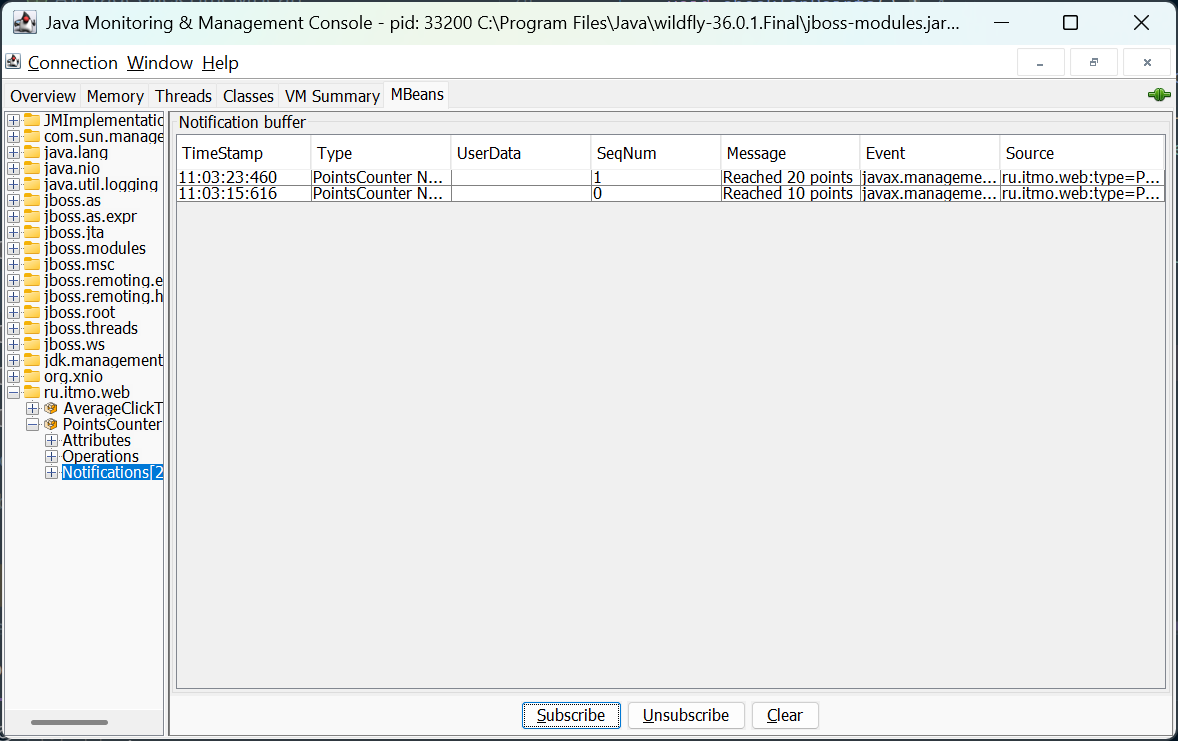
\includegraphics[width=1\linewidth]{jconsole/notifications}
		\caption{Уведомления от PointsCounter при достижении числа точек, кратного 10}
		\label{fig:notifications}
	\end{figure}
	
	\subsection{Определение \texttt{Java Language Specification}}
	
	\begin{figure}[H]
		\centering
		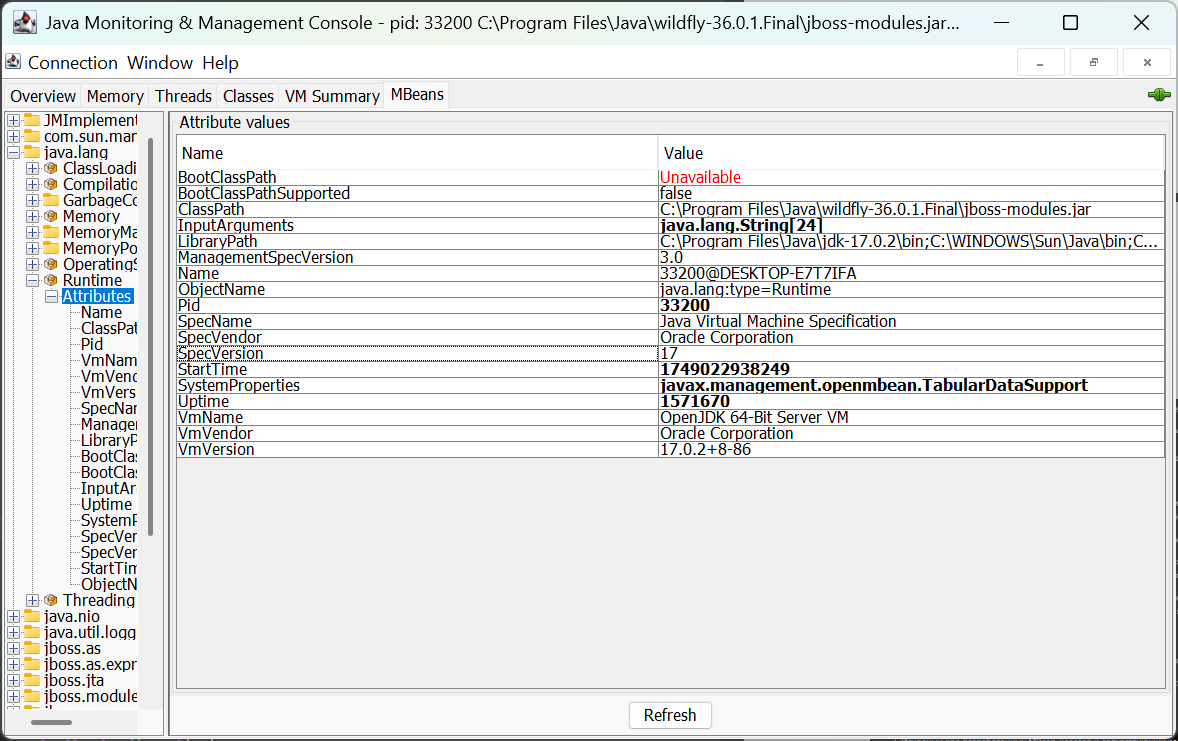
\includegraphics[width=1\linewidth]{jconsole/JLS_version}
		\caption{Определение версии Java Language Specification в JConsole}
		\label{fig:jlsversion}
	\end{figure}

	\newpage
	
	\section{Мониторинг и профилирование с помощью VisualVM}
	
	\subsection{Графики изменения показаний MBean-классов во времени}
	
	\begin{figure}[H]
		\centering
		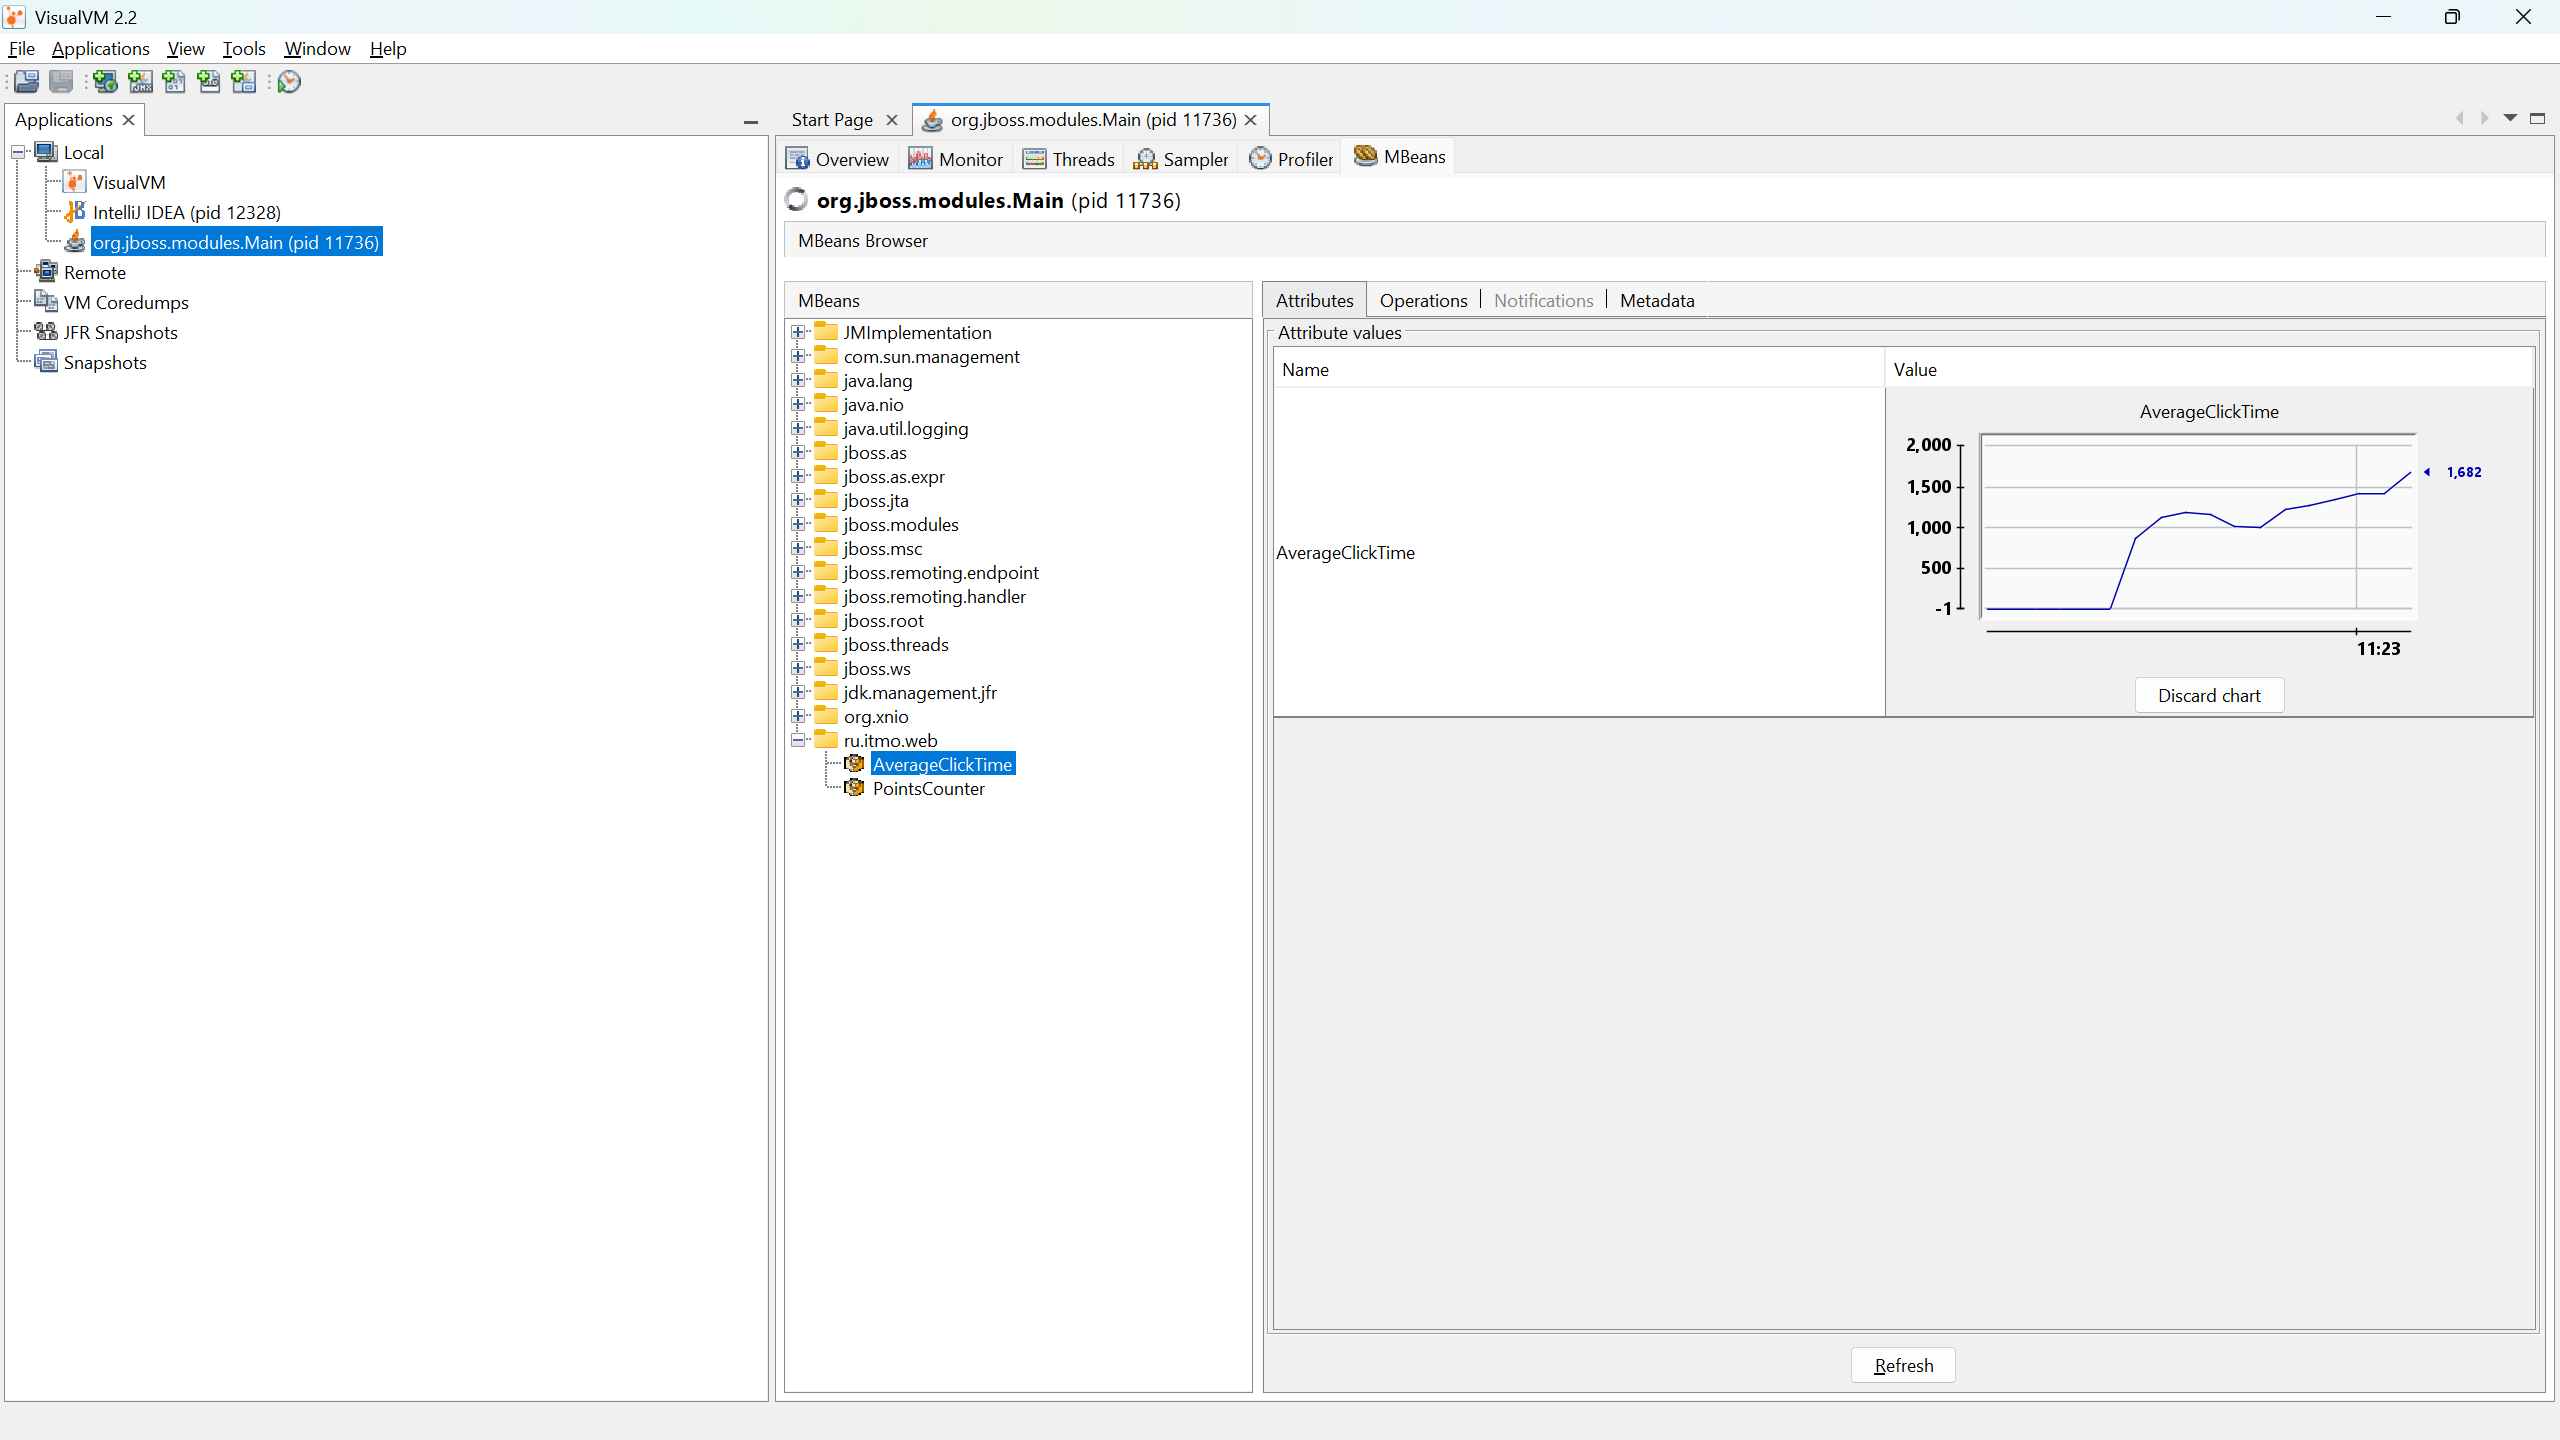
\includegraphics[width=1\linewidth]{visualvm/average_time_graphic}
		\caption{График изменения среднего времени между кликами в VisualVM}
		\label{fig:averagetimegraphic}
	\end{figure}
	
	\begin{figure}[H]
		\centering
		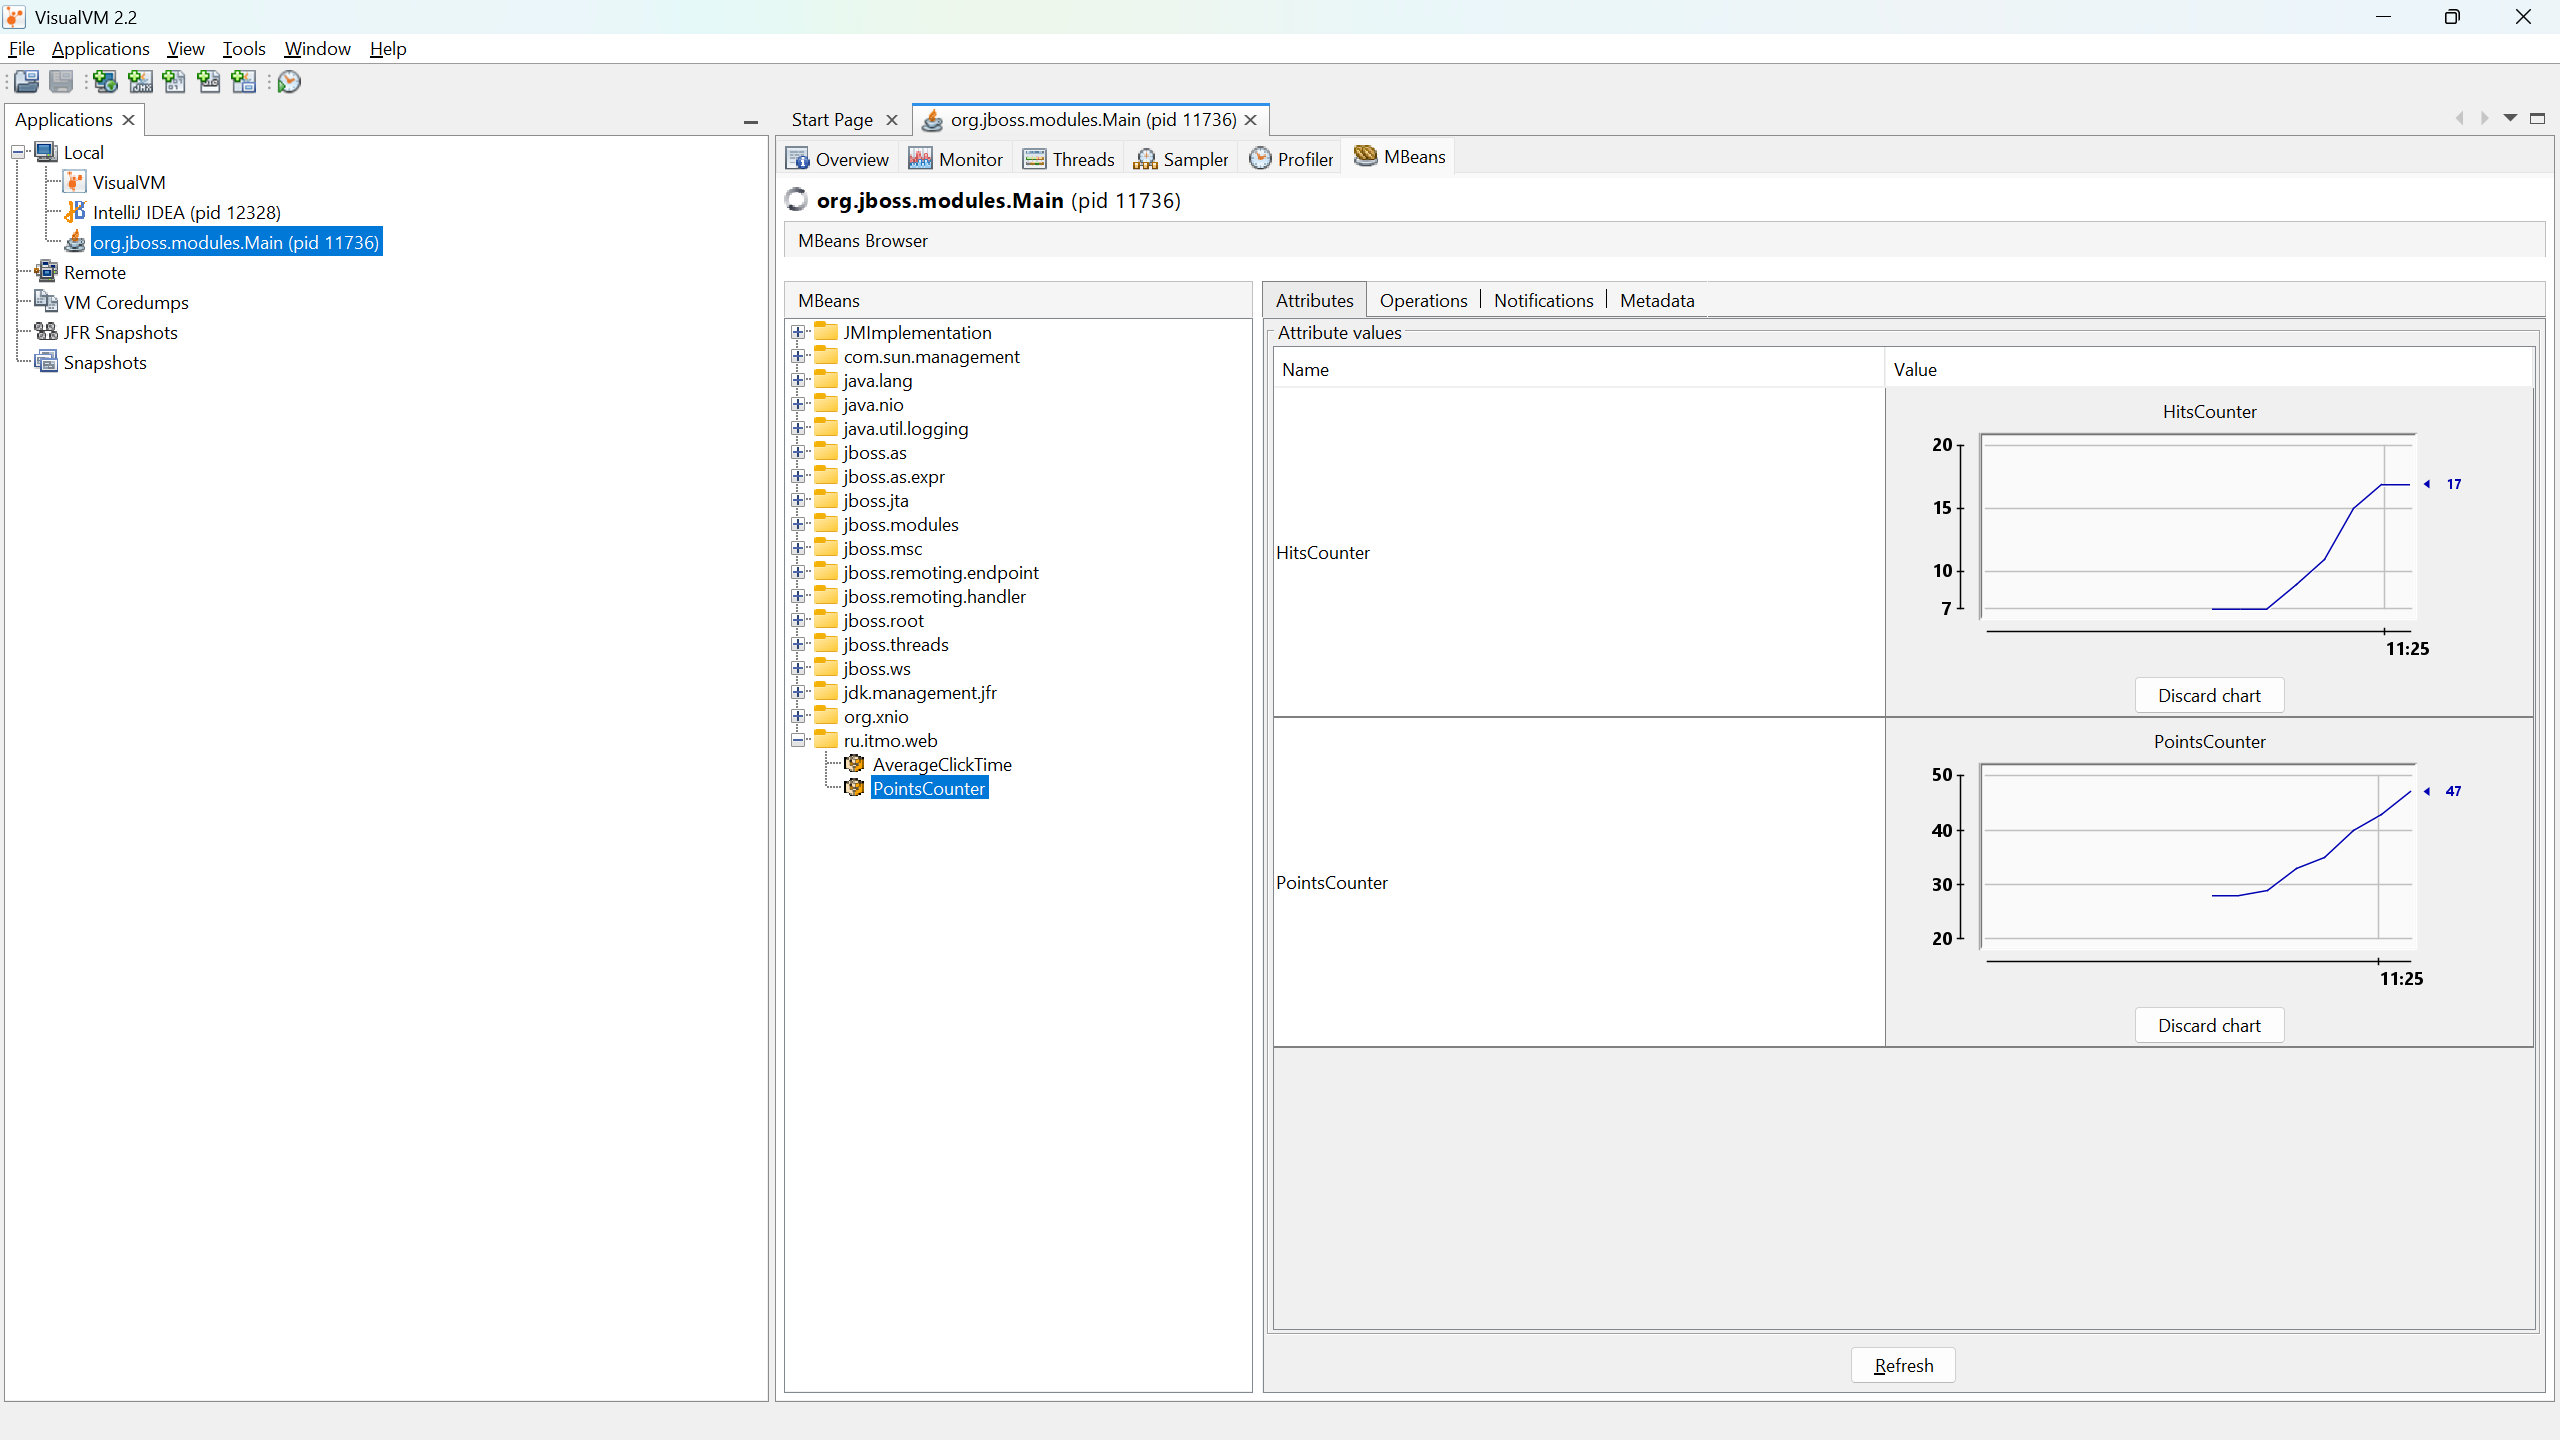
\includegraphics[width=1\linewidth]{visualvm/point_counter_graphics}
		\caption{График изменения числа точек и попаданий в VisualVM}
		\label{fig:pointcountergraphics}
	\end{figure}
	
	\subsection{Определение класса с наибольшим использованием памяти}
	
	\begin{figure}[H]
		\centering
		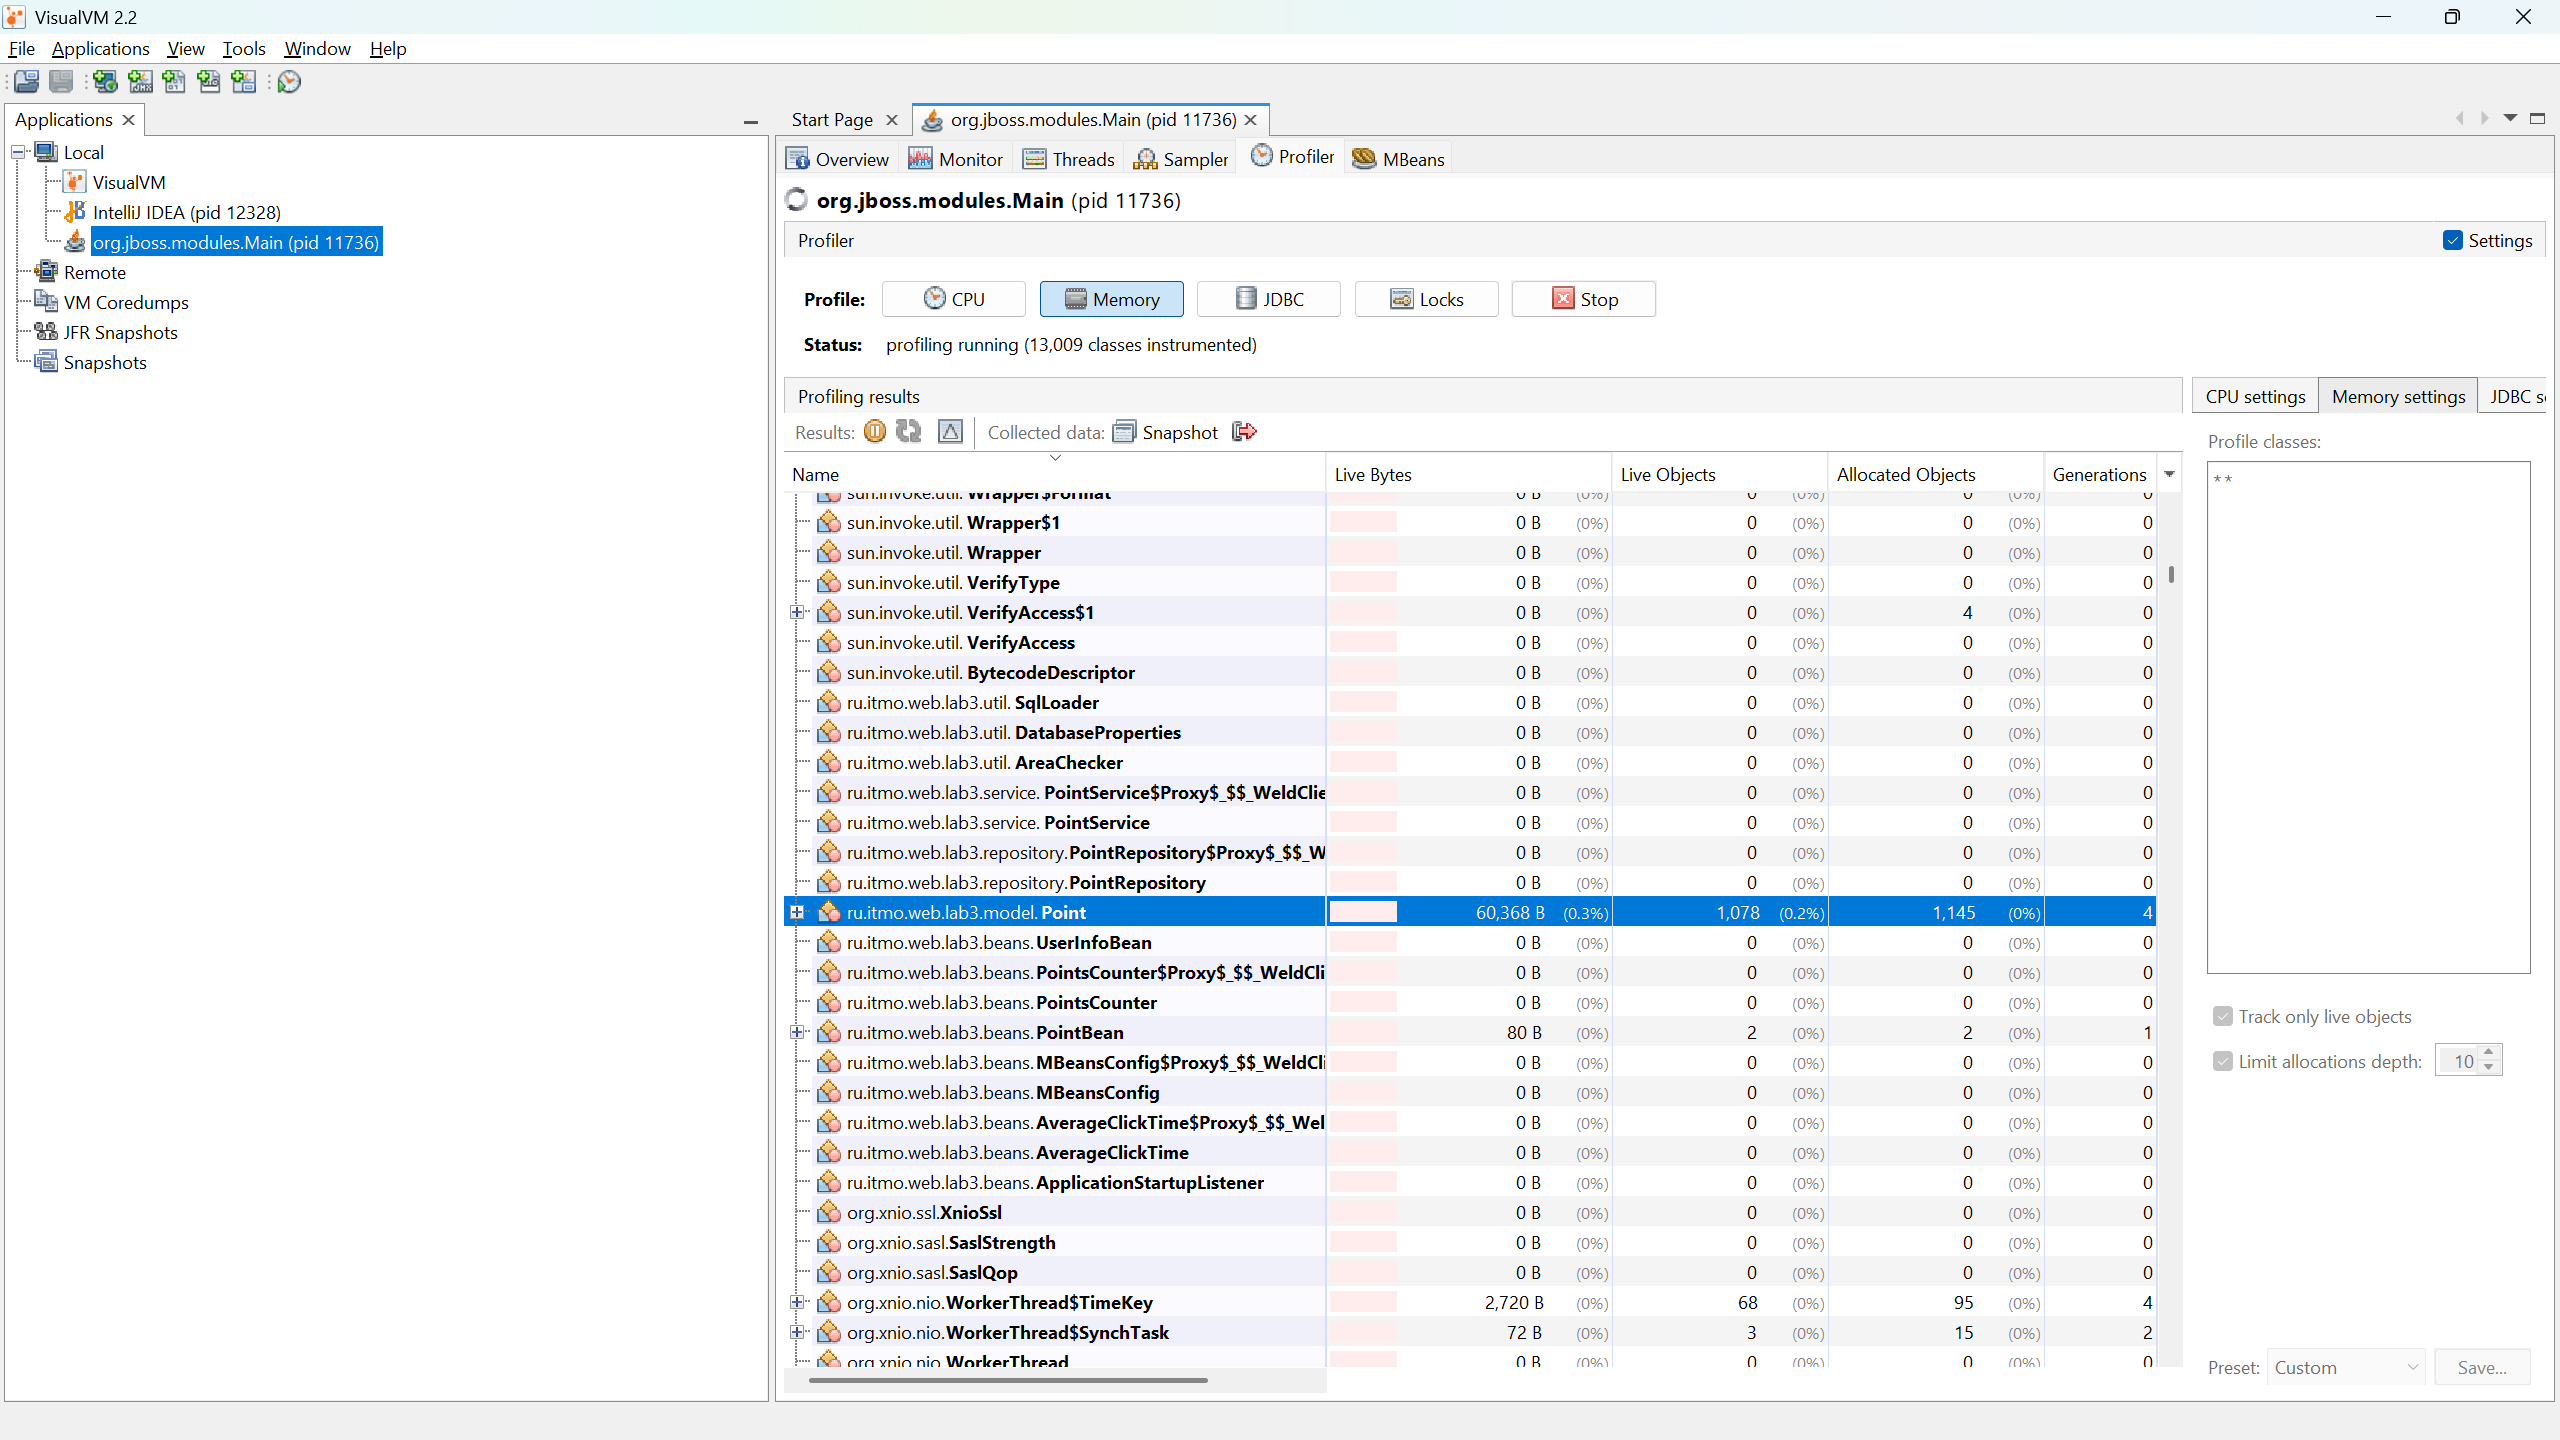
\includegraphics[width=1\linewidth]{visualvm/max_memory_usage_user_class}
		\caption{Класс Point, занимающий наибольший объем памяти в куче}
		\label{fig:maxmemoryusageuserclass}
	\end{figure}
	
	\begin{figure}[H]
		\centering
		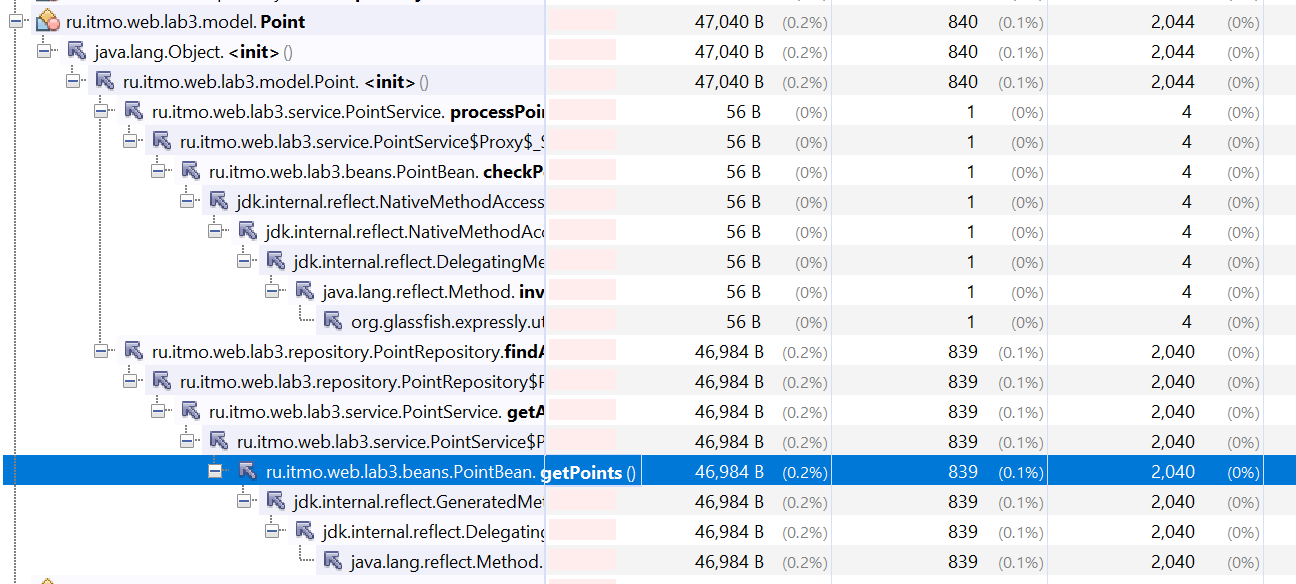
\includegraphics[width=1\linewidth]{visualvm/classes_that_uses_points}
		\caption{Класс, содержащий объекты Point (обращение к базе данных)}
		\label{fig:classesthatusespoints}
	\end{figure}
	
	\begin{figure}[H]
		\centering
		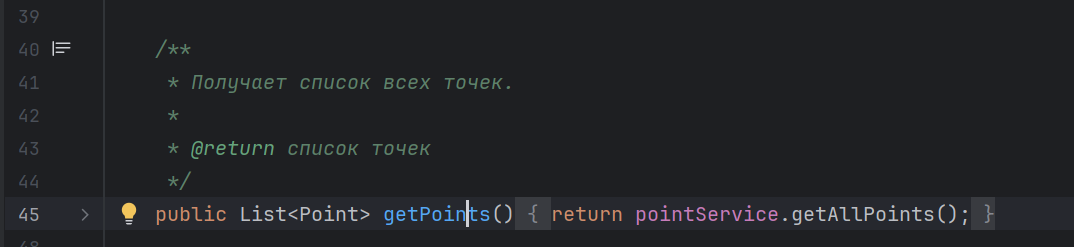
\includegraphics[width=1\linewidth]{visualvm/method_that_gets_all_points}
		\caption{Метод, загружающий все точки из базы данных}
		\label{fig:methodthatgetsallpoints}
	\end{figure}
	
	
	\section{Локализация и устранение проблем производительности}
	
	Запустим приложение и откроем в visualvm
	
	\begin{figure}[H]
		\centering
		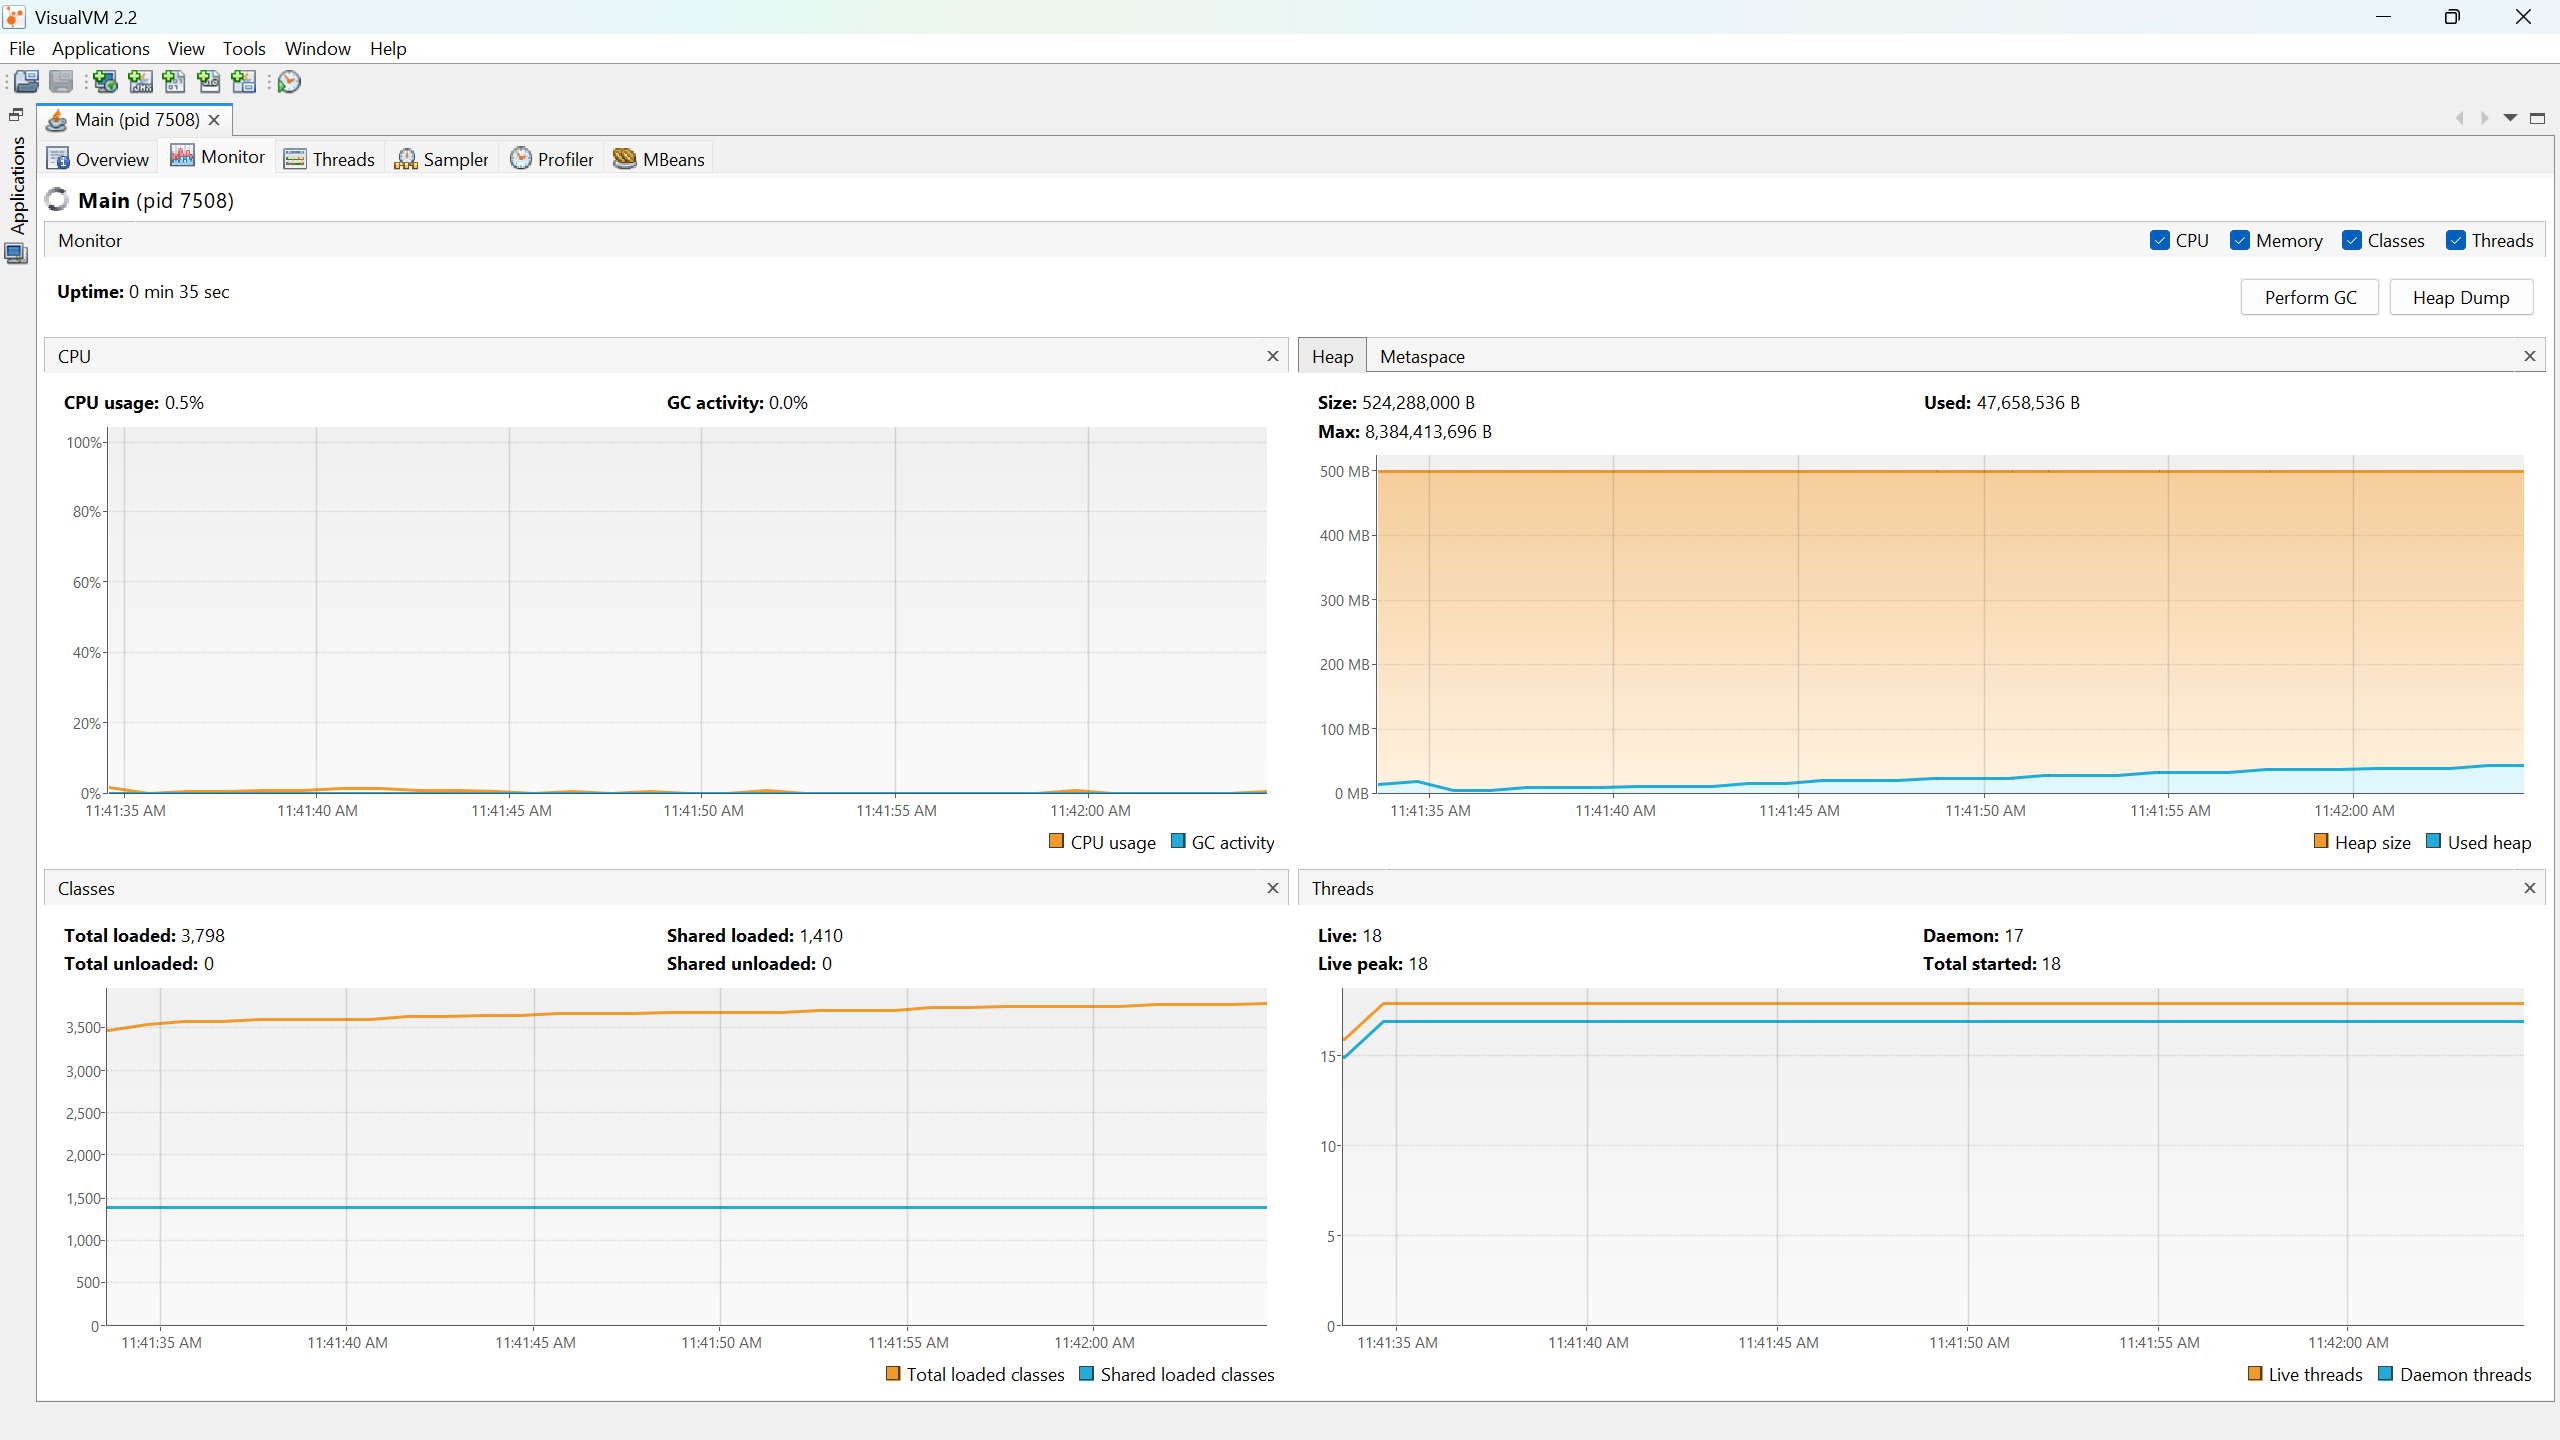
\includegraphics[width=1\linewidth]{visualvm/app_in_visualvm}
		\caption{Запуск приложения в VisualVM для мониторинга}
		\label{fig:appinvisualvm}
	\end{figure}
	
	Ограничим память и уберём Thread.sleep, чтобы ускорить отправку запросов и тестирование
	
	\begin{figure}[H]
		\centering
		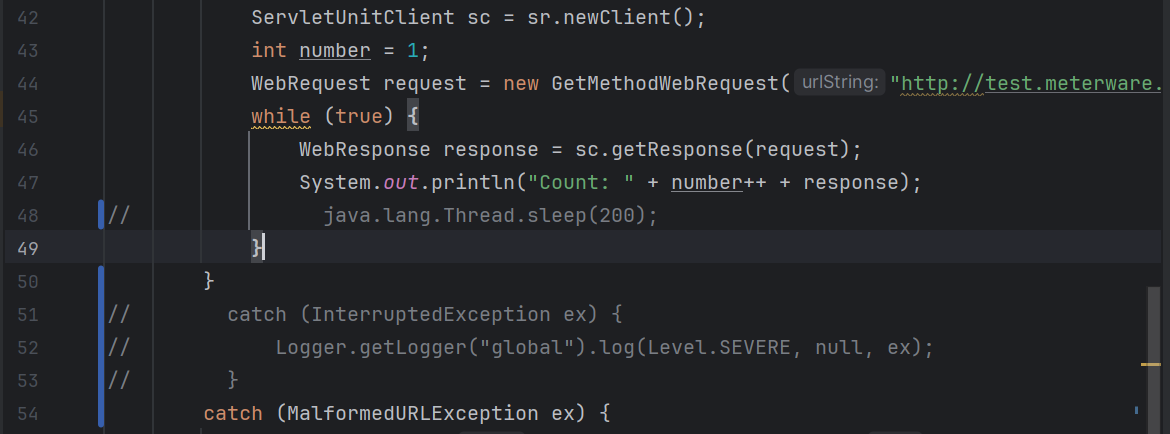
\includegraphics[width=1\linewidth]{visualvm/commented_thread_sleep}
		\caption{Удаление Thread.sleep для ускорения тестирования}
		\label{fig:commentedthreadsleep}
	\end{figure}
	\begin{figure}[H]
		\centering
		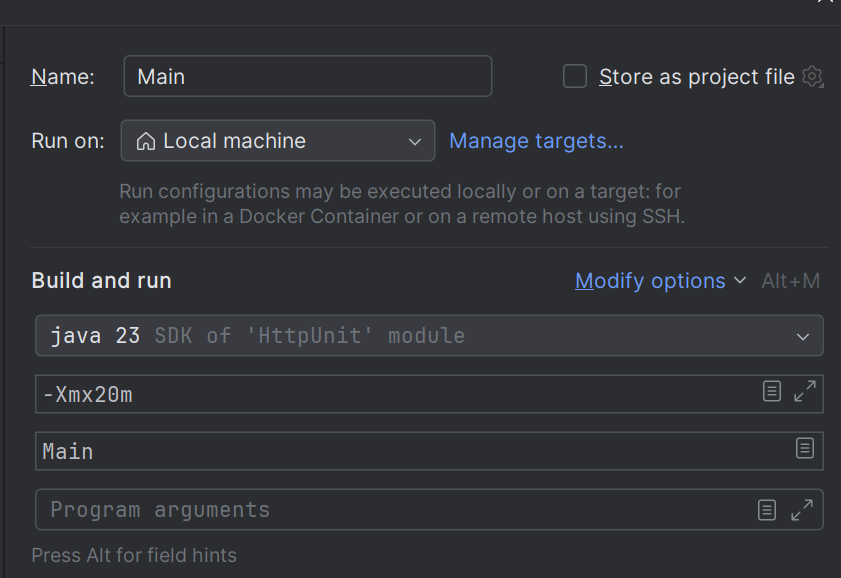
\includegraphics[width=1\linewidth]{visualvm/added_xmx_20m}
		\caption{Ограничение памяти JVM до 20 МБ с параметром -Xmx20m}
		\label{fig:addedxmx20m}
	\end{figure}
	
	\begin{figure}[H]
		\centering
		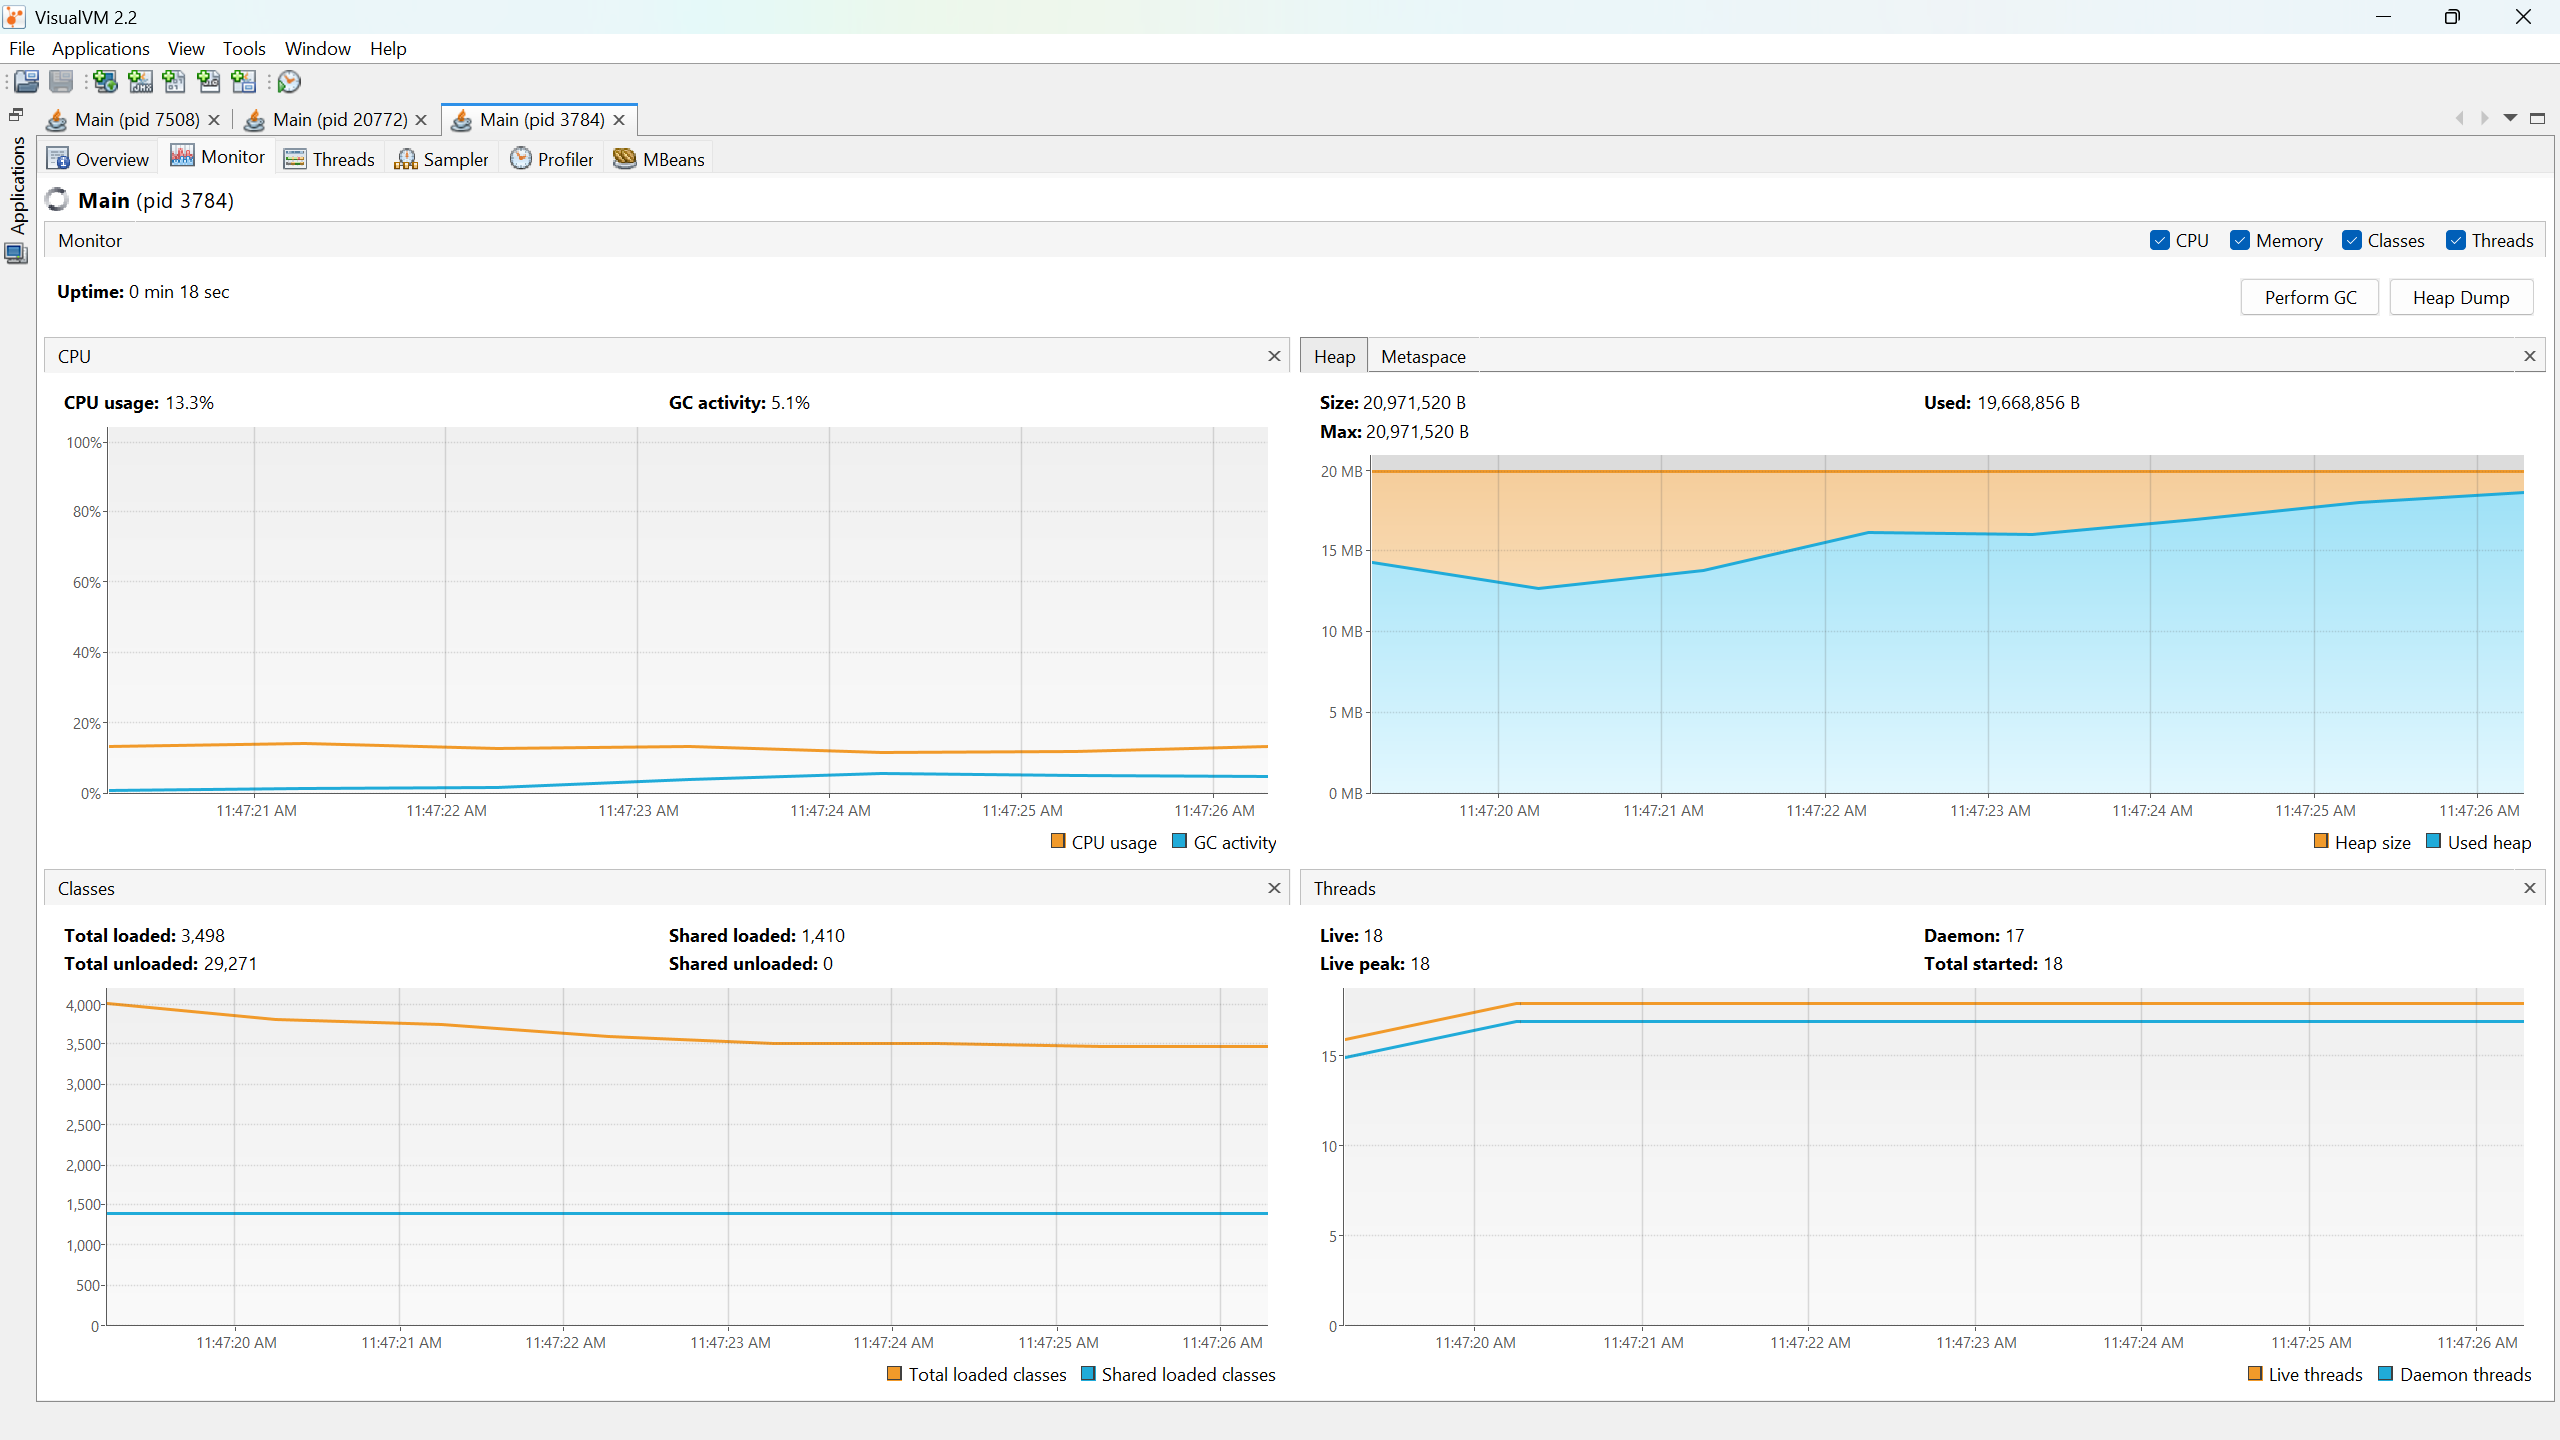
\includegraphics[width=1\linewidth]{visualvm/raise_of_heap_size}
		\caption{Рост использования кучи до завершения программы за 20 секунд}
		\label{fig:raiseofheapsize}
	\end{figure}
	\begin{figure}[H]
		\centering
		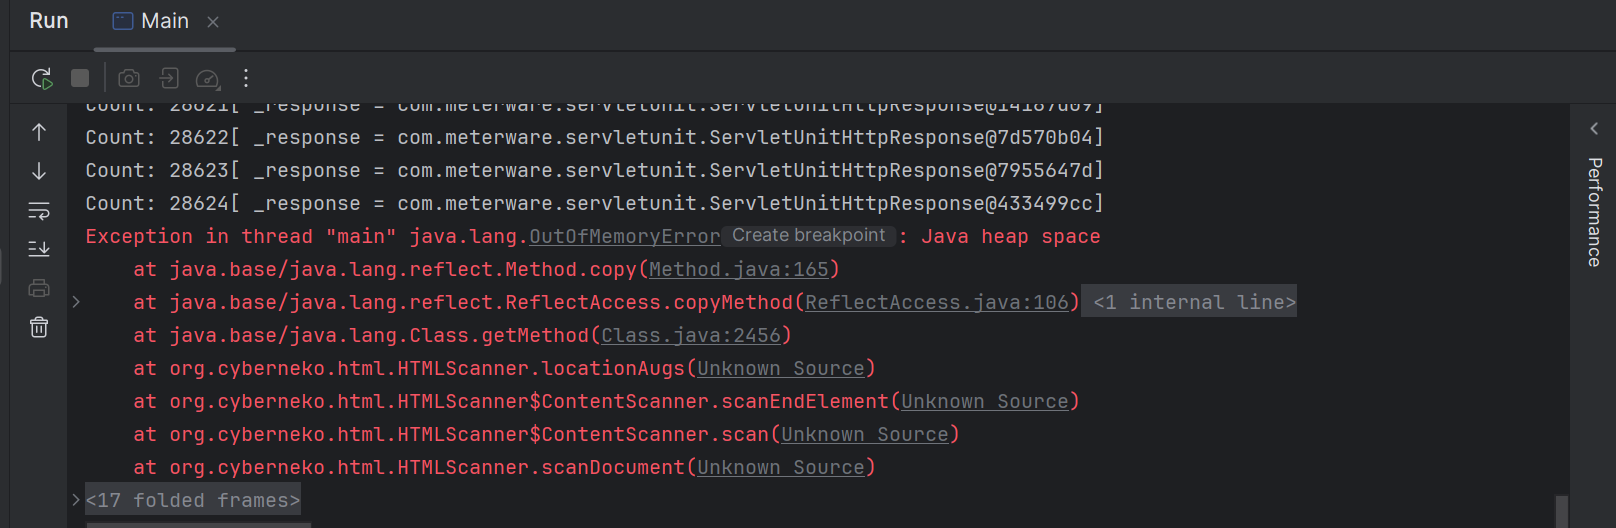
\includegraphics[width=1\linewidth]{visualvm/out_of_memmory_heap_size_error}
		\caption{Ошибка OutOfMemoryError при исчерпании памяти}
		\label{fig:outofmemmoryheapsizeerror}
	\end{figure}
	
	Увеличим память до 25 и сделаем heap dump когда heap накопится, делаем ещё несколько heap dump через некоторое время
	
	\begin{figure}[H]
		\centering
		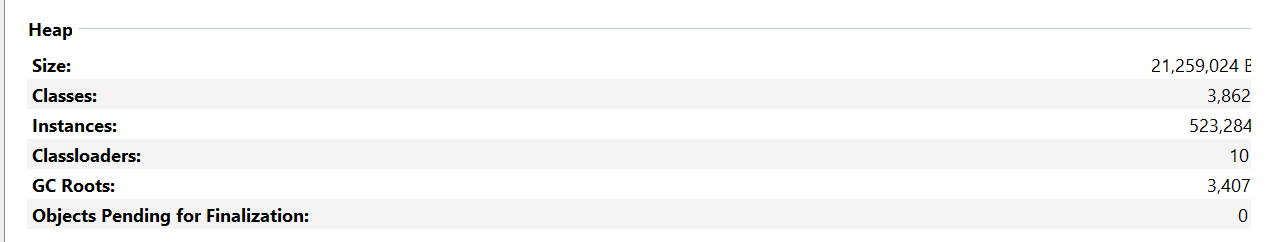
\includegraphics[width=0.5\linewidth]{visualvm/Dump1}
		\caption{Heap dump 1: начальное состояние кучи при увеличении памяти до 25 МБ}
		\label{fig:dump1}
	\end{figure}
	\begin{figure}[H]
		\centering
		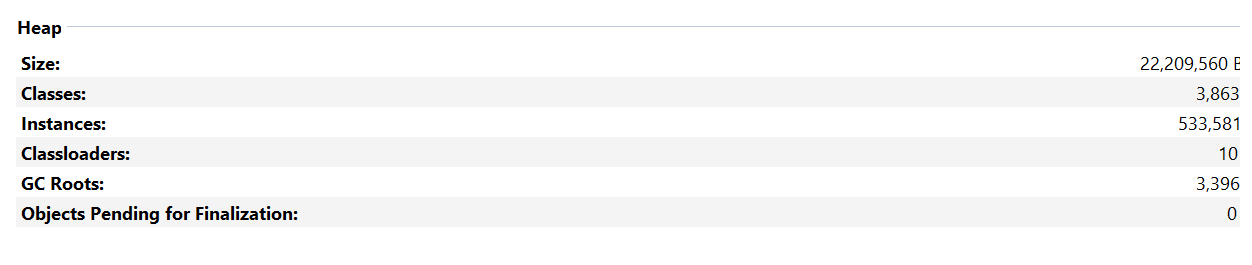
\includegraphics[width=0.5\linewidth]{visualvm/Dump2}
		\caption{Heap dump 2: промежуточное состояние кучи через несколько секунд}
		\label{fig:dump2}
	\end{figure}
	\begin{figure}[H]
		\centering
		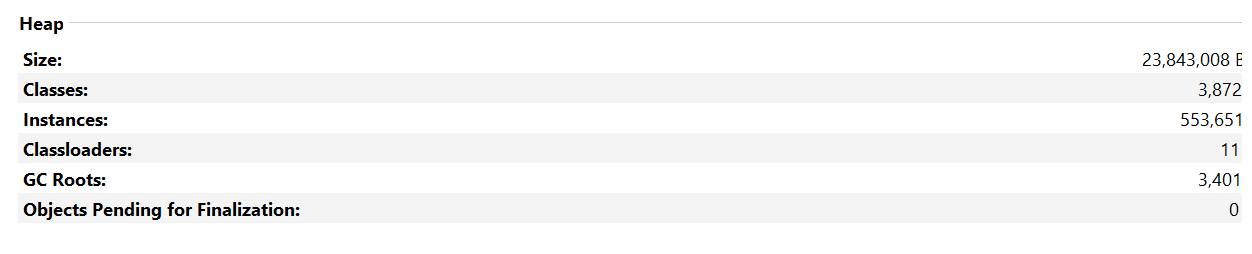
\includegraphics[width=0.5\linewidth]{visualvm/Dump3}
		\caption{Heap dump 3: финальное состояние кучи с накоплением объектов}
		\label{fig:dump3}
	\end{figure}
	
	Замечаем увеличение количества инстансов со временем, открываем последний дамп и смотрим какие объекты создаются
	
	\begin{figure}[H]
		\centering
		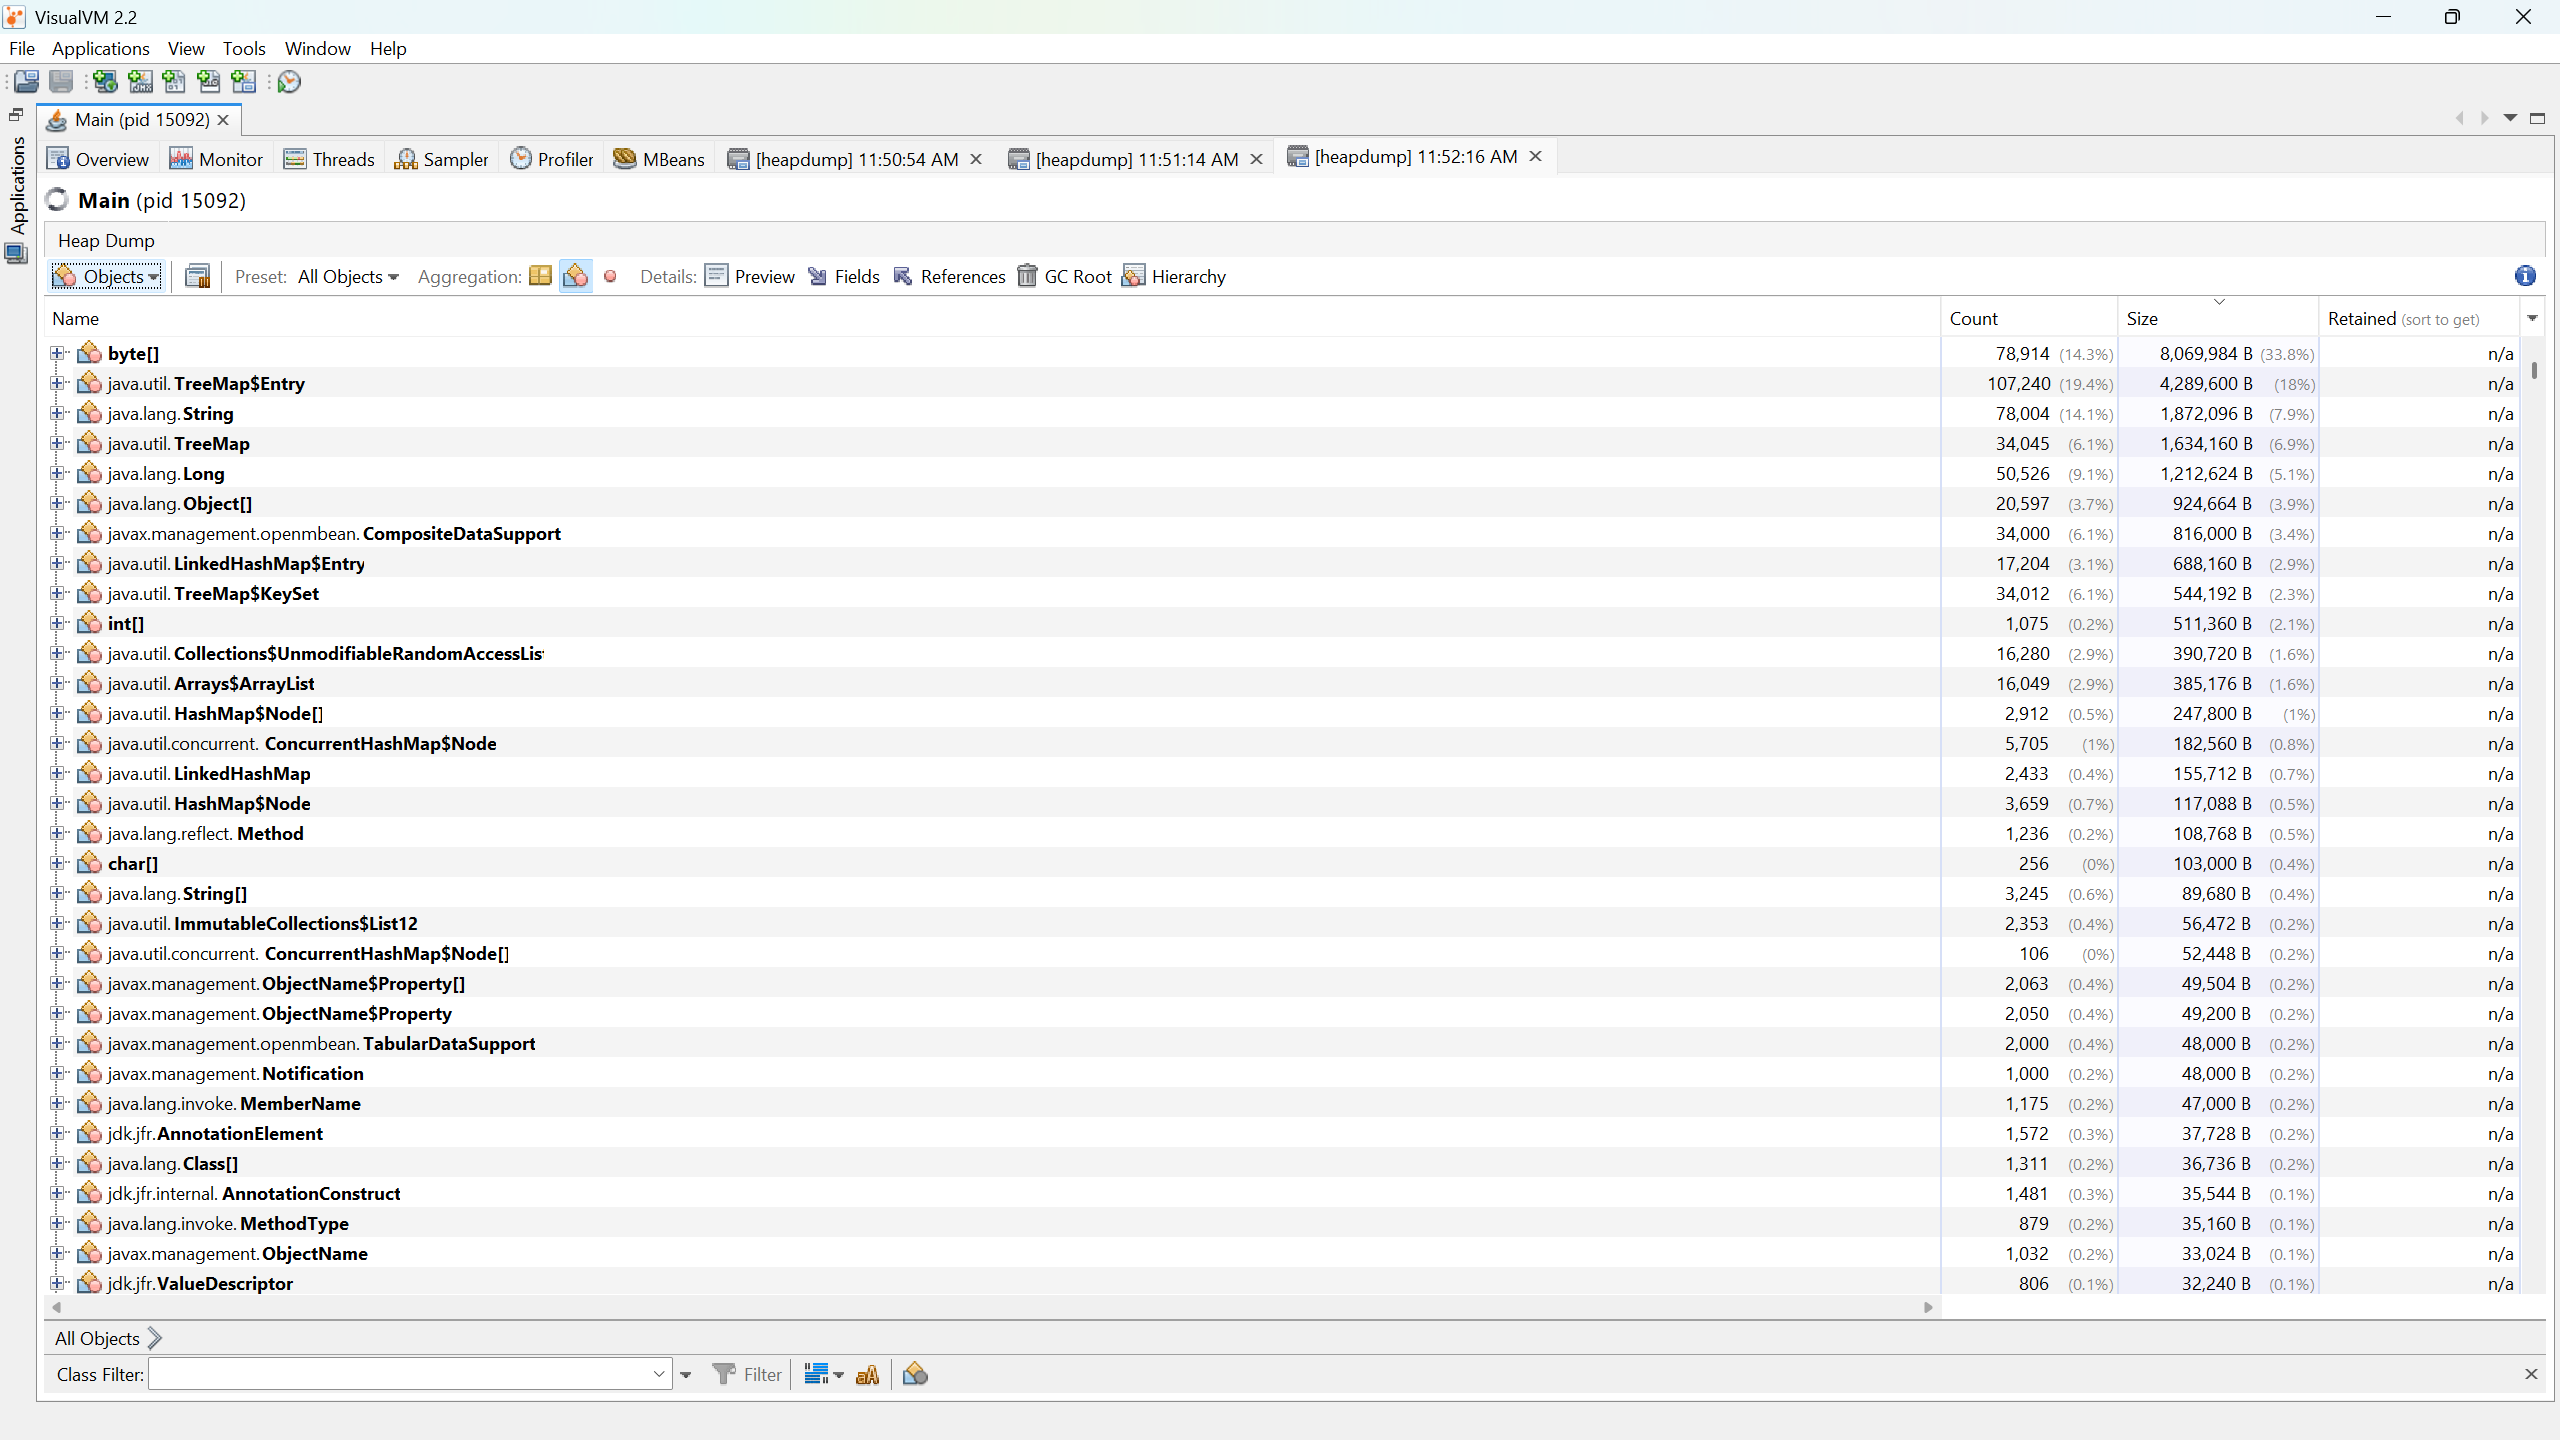
\includegraphics[width=1\linewidth]{visualvm/objects}
		\caption{Анализ объектов в последнем heap dump}
		\label{fig:objects}
	\end{figure}
	
	Недолго просмотрев объекты занимающие больше всего памяти замечаем повторяющиеся ошибки
	
	\begin{figure}[H]
		\centering
		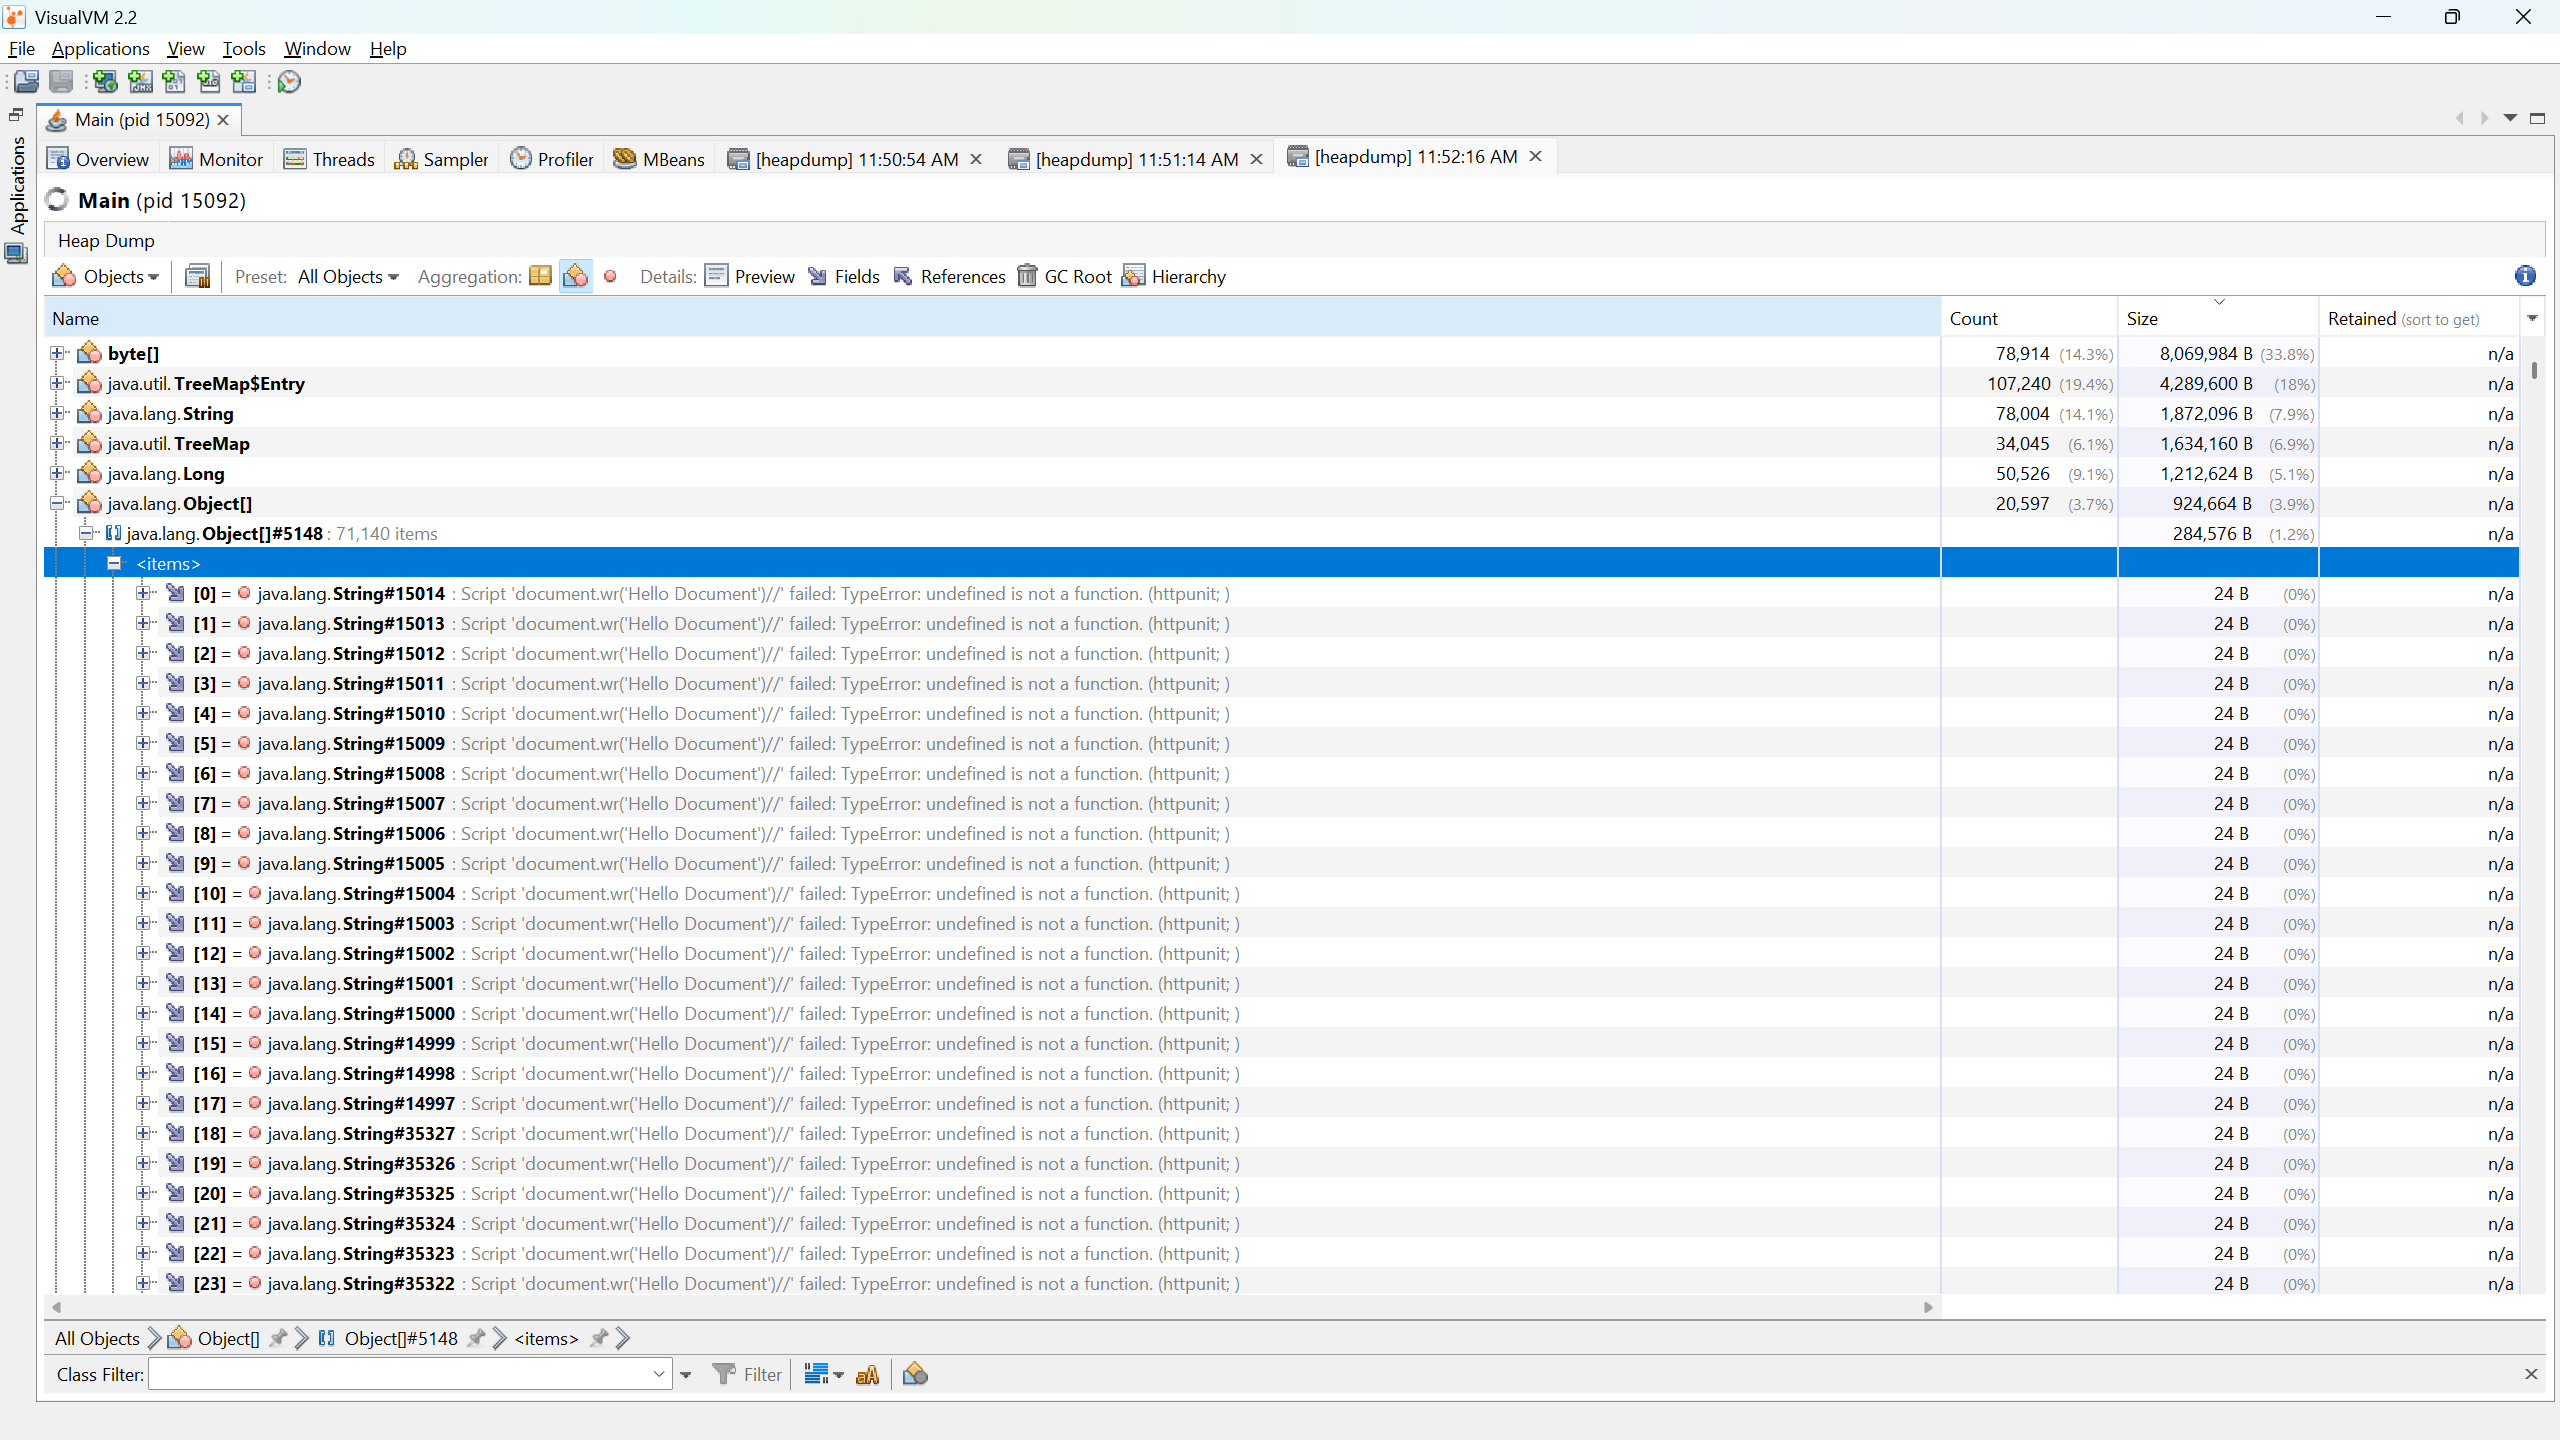
\includegraphics[width=1\linewidth]{visualvm/errors}
		\caption{Обнаружение накопления ошибок в heap dump}
		\label{fig:errors}
	\end{figure}
	
	Смотрим класс их хранения
	
	\begin{figure}[H]
		\centering
		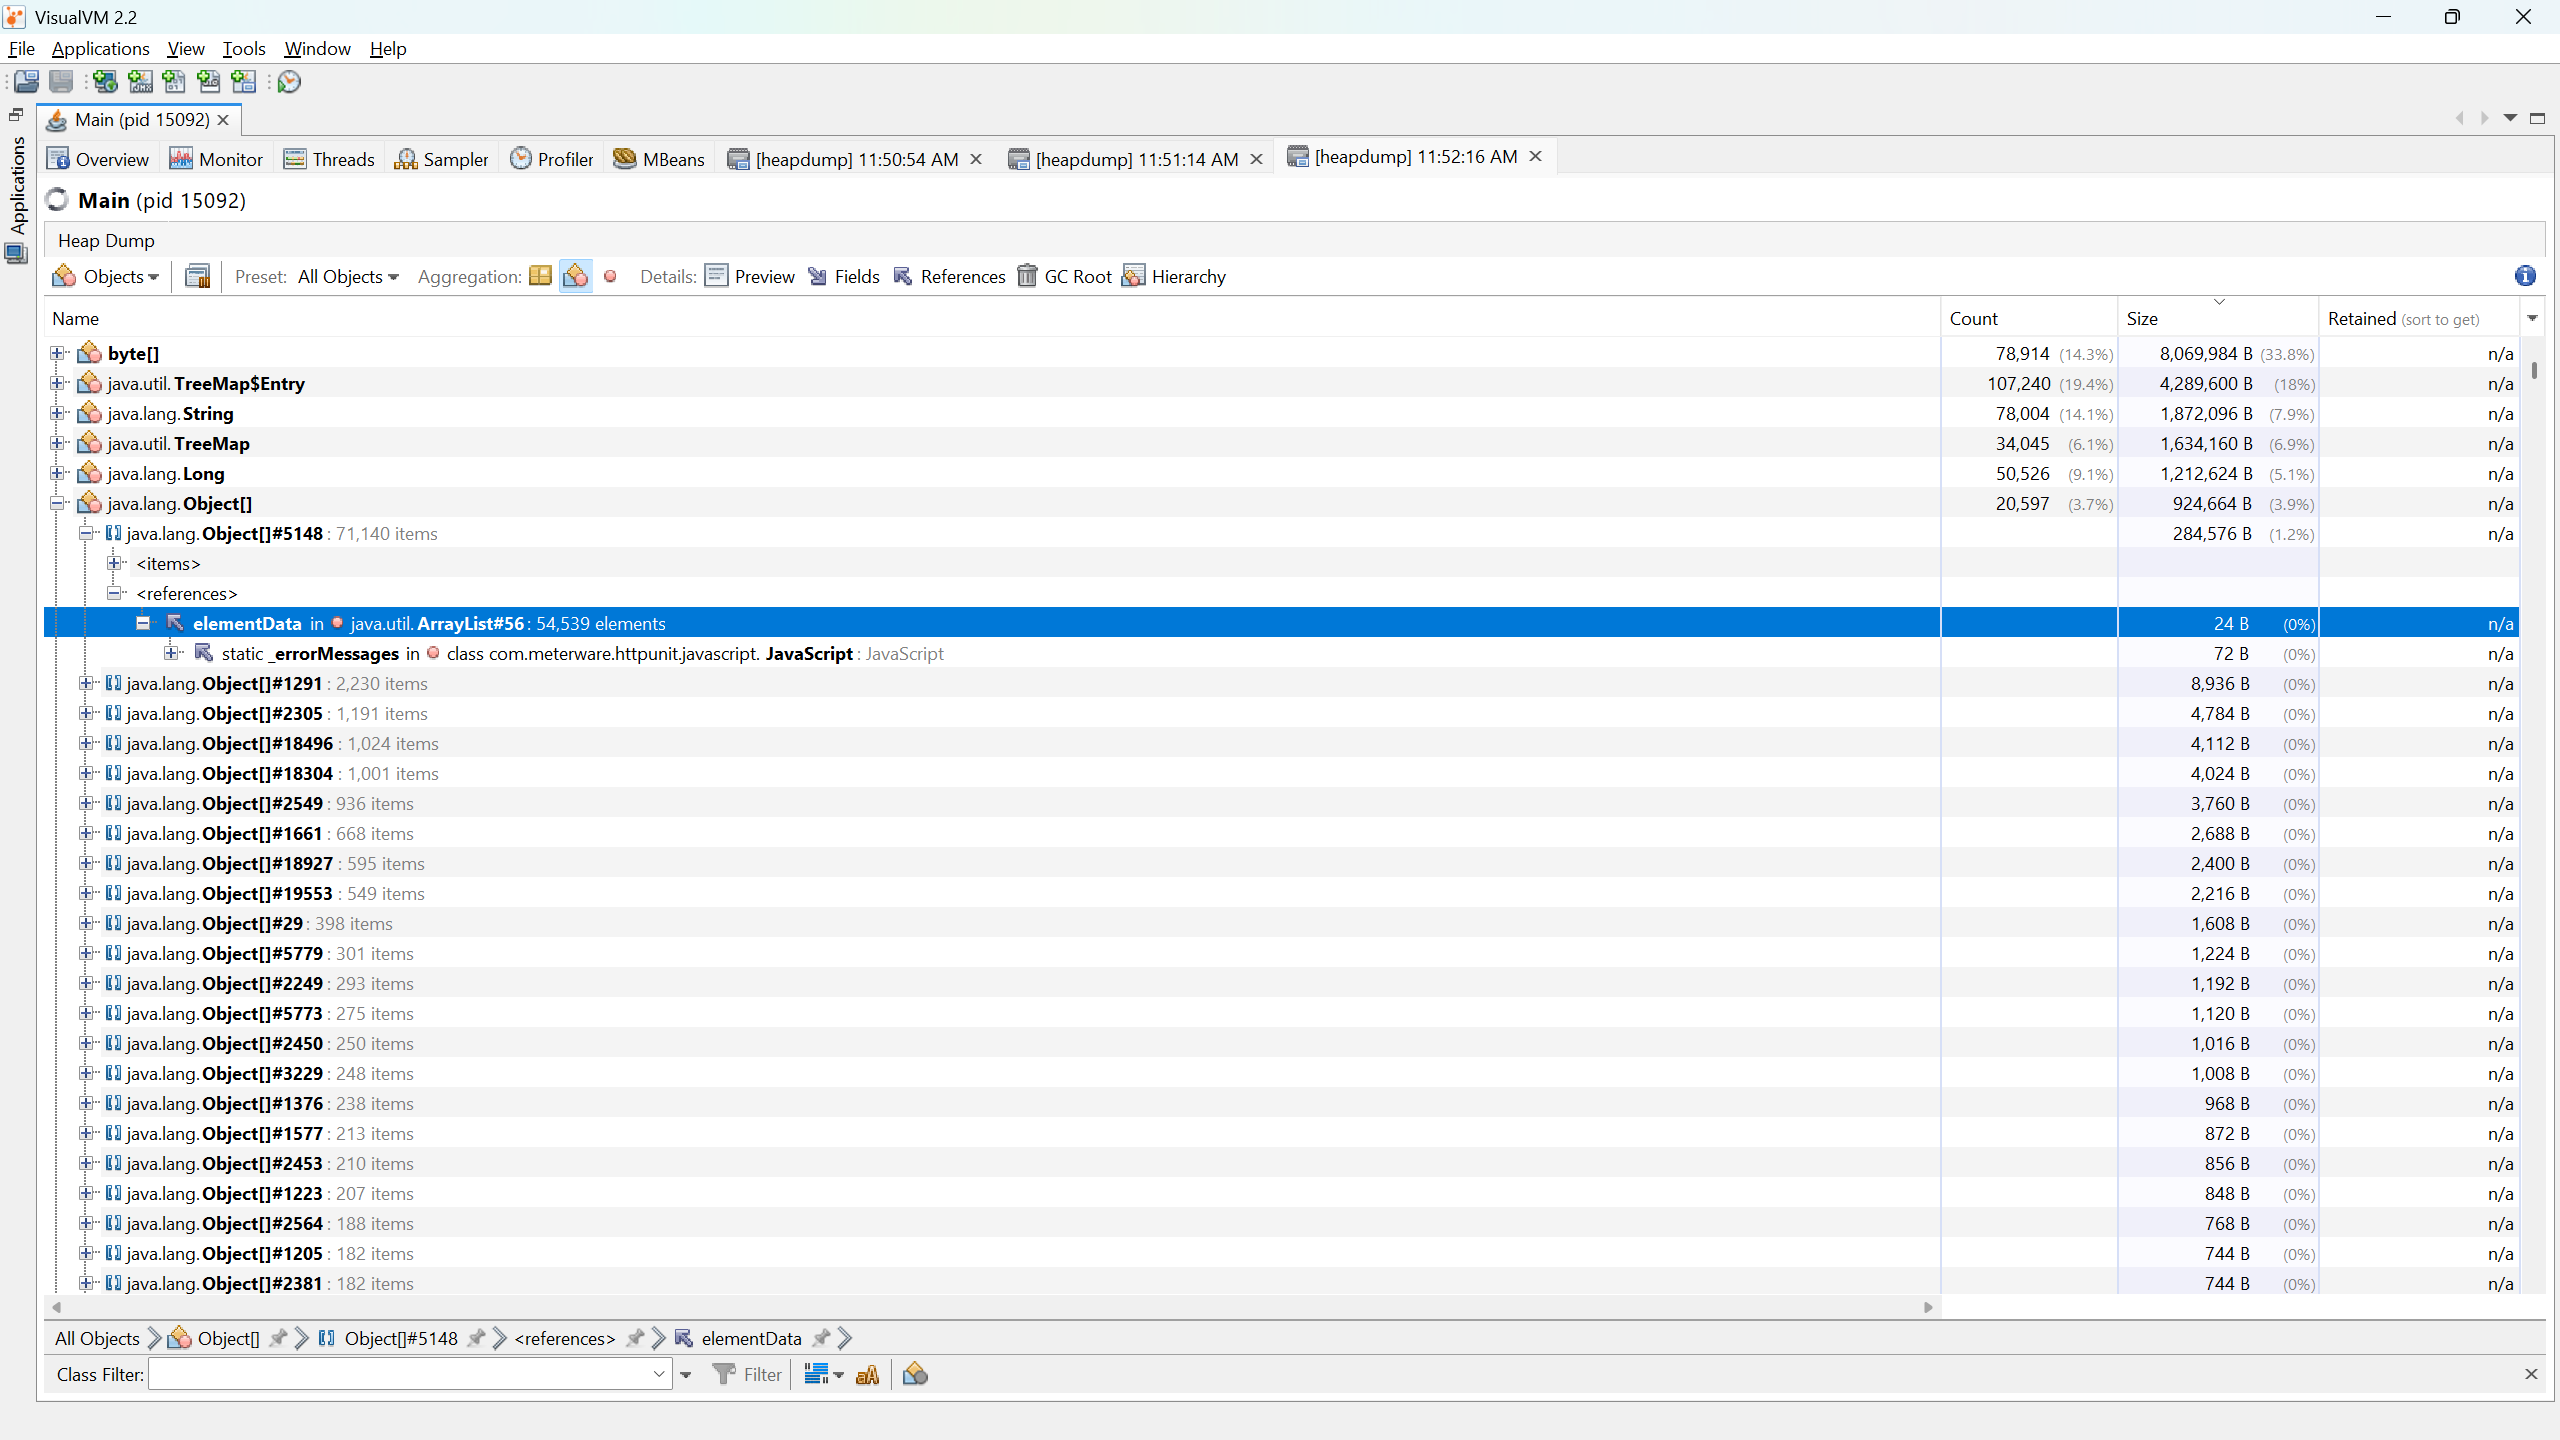
\includegraphics[width=1\linewidth]{visualvm/errors_locate}
		\caption{Локализация ошибок в ArrayList класса JavaScript}
		\label{fig:errorslocate}
	\end{figure}
	
	ArrayList хранит все эти ошибки и находится в классе JavaScript, заходим в него и смотрим поля класса
	
	\begin{figure}[H]
		\centering
		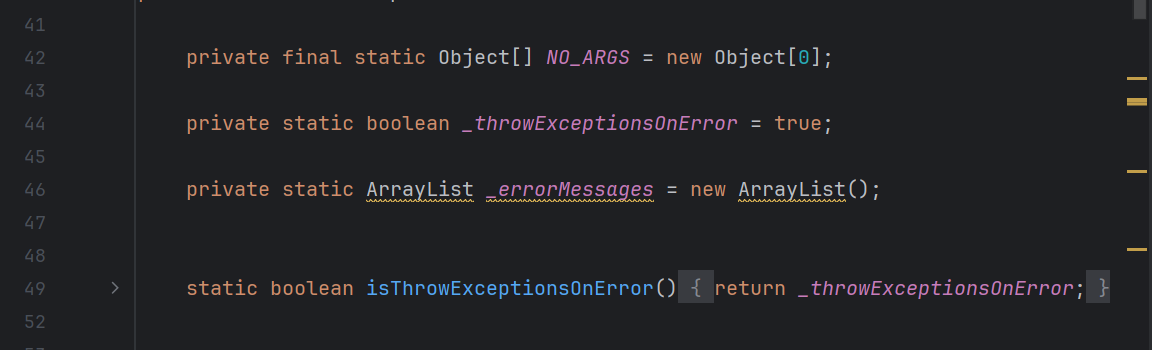
\includegraphics[width=1\linewidth]{visualvm/java_script_fields}
		\caption{Поля класса JavaScript, содержащие ArrayList}
		\label{fig:javascriptfields}
	\end{figure}
	
	Видим только 1 ArrayList, смотрим где он дополняется и очищается
	
	\begin{figure}[H]
		\centering
		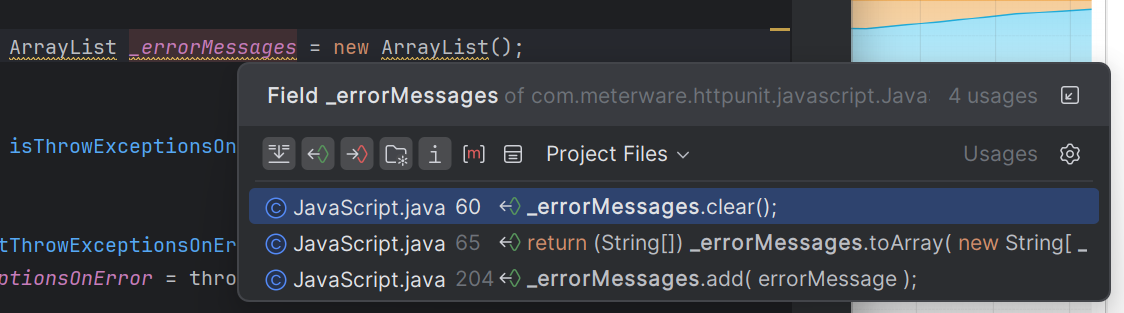
\includegraphics[width=1\linewidth]{visualvm/array_list_methods}
		\caption{Методы добавления элементов в ArrayList}
		\label{fig:arraylistmethods}
	\end{figure}
	
	\begin{figure}[H]
		\centering
		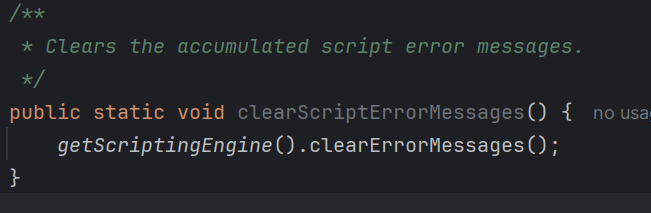
\includegraphics[width=1\linewidth]{visualvm/array_list_clear}
		\caption{Метод очистки ArrayList, который не вызывался}
		\label{fig:arraylistclear}
	\end{figure}
	
	Обнаруживаем, что очистка не вызывается в коде, добавляем самое простое решение, очистку в цикле запросов Main
	
	\begin{figure}[H]
		\centering
		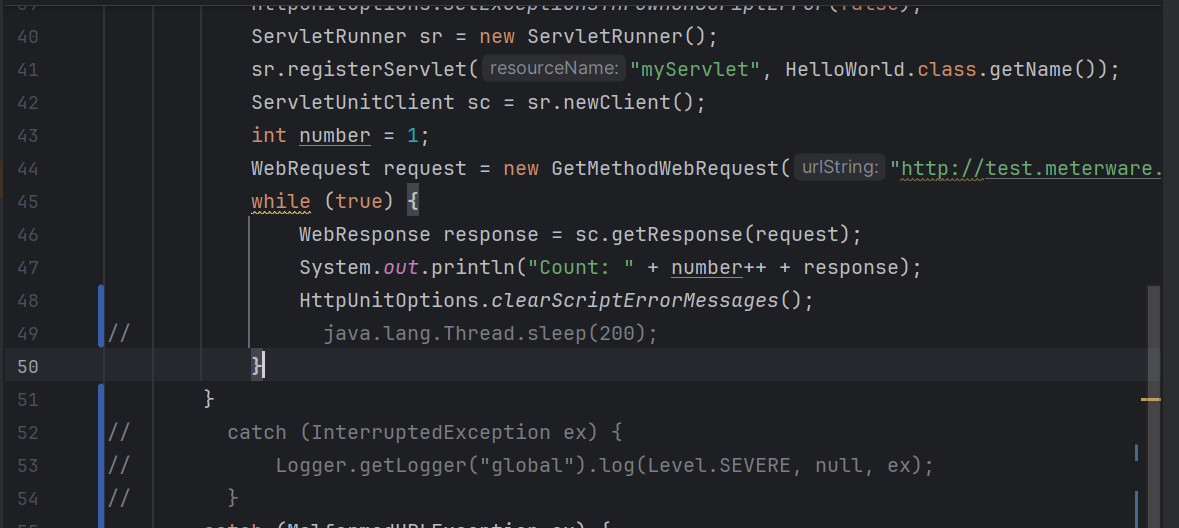
\includegraphics[width=1\linewidth]{visualvm/using_clear}
		\caption{Добавление очистки ArrayList в цикл запросов}
		\label{fig:usingclear}
	\end{figure}
	
	Снова запускаем с кучей размера 20 мб
	
	\begin{figure}[H]
		\centering
		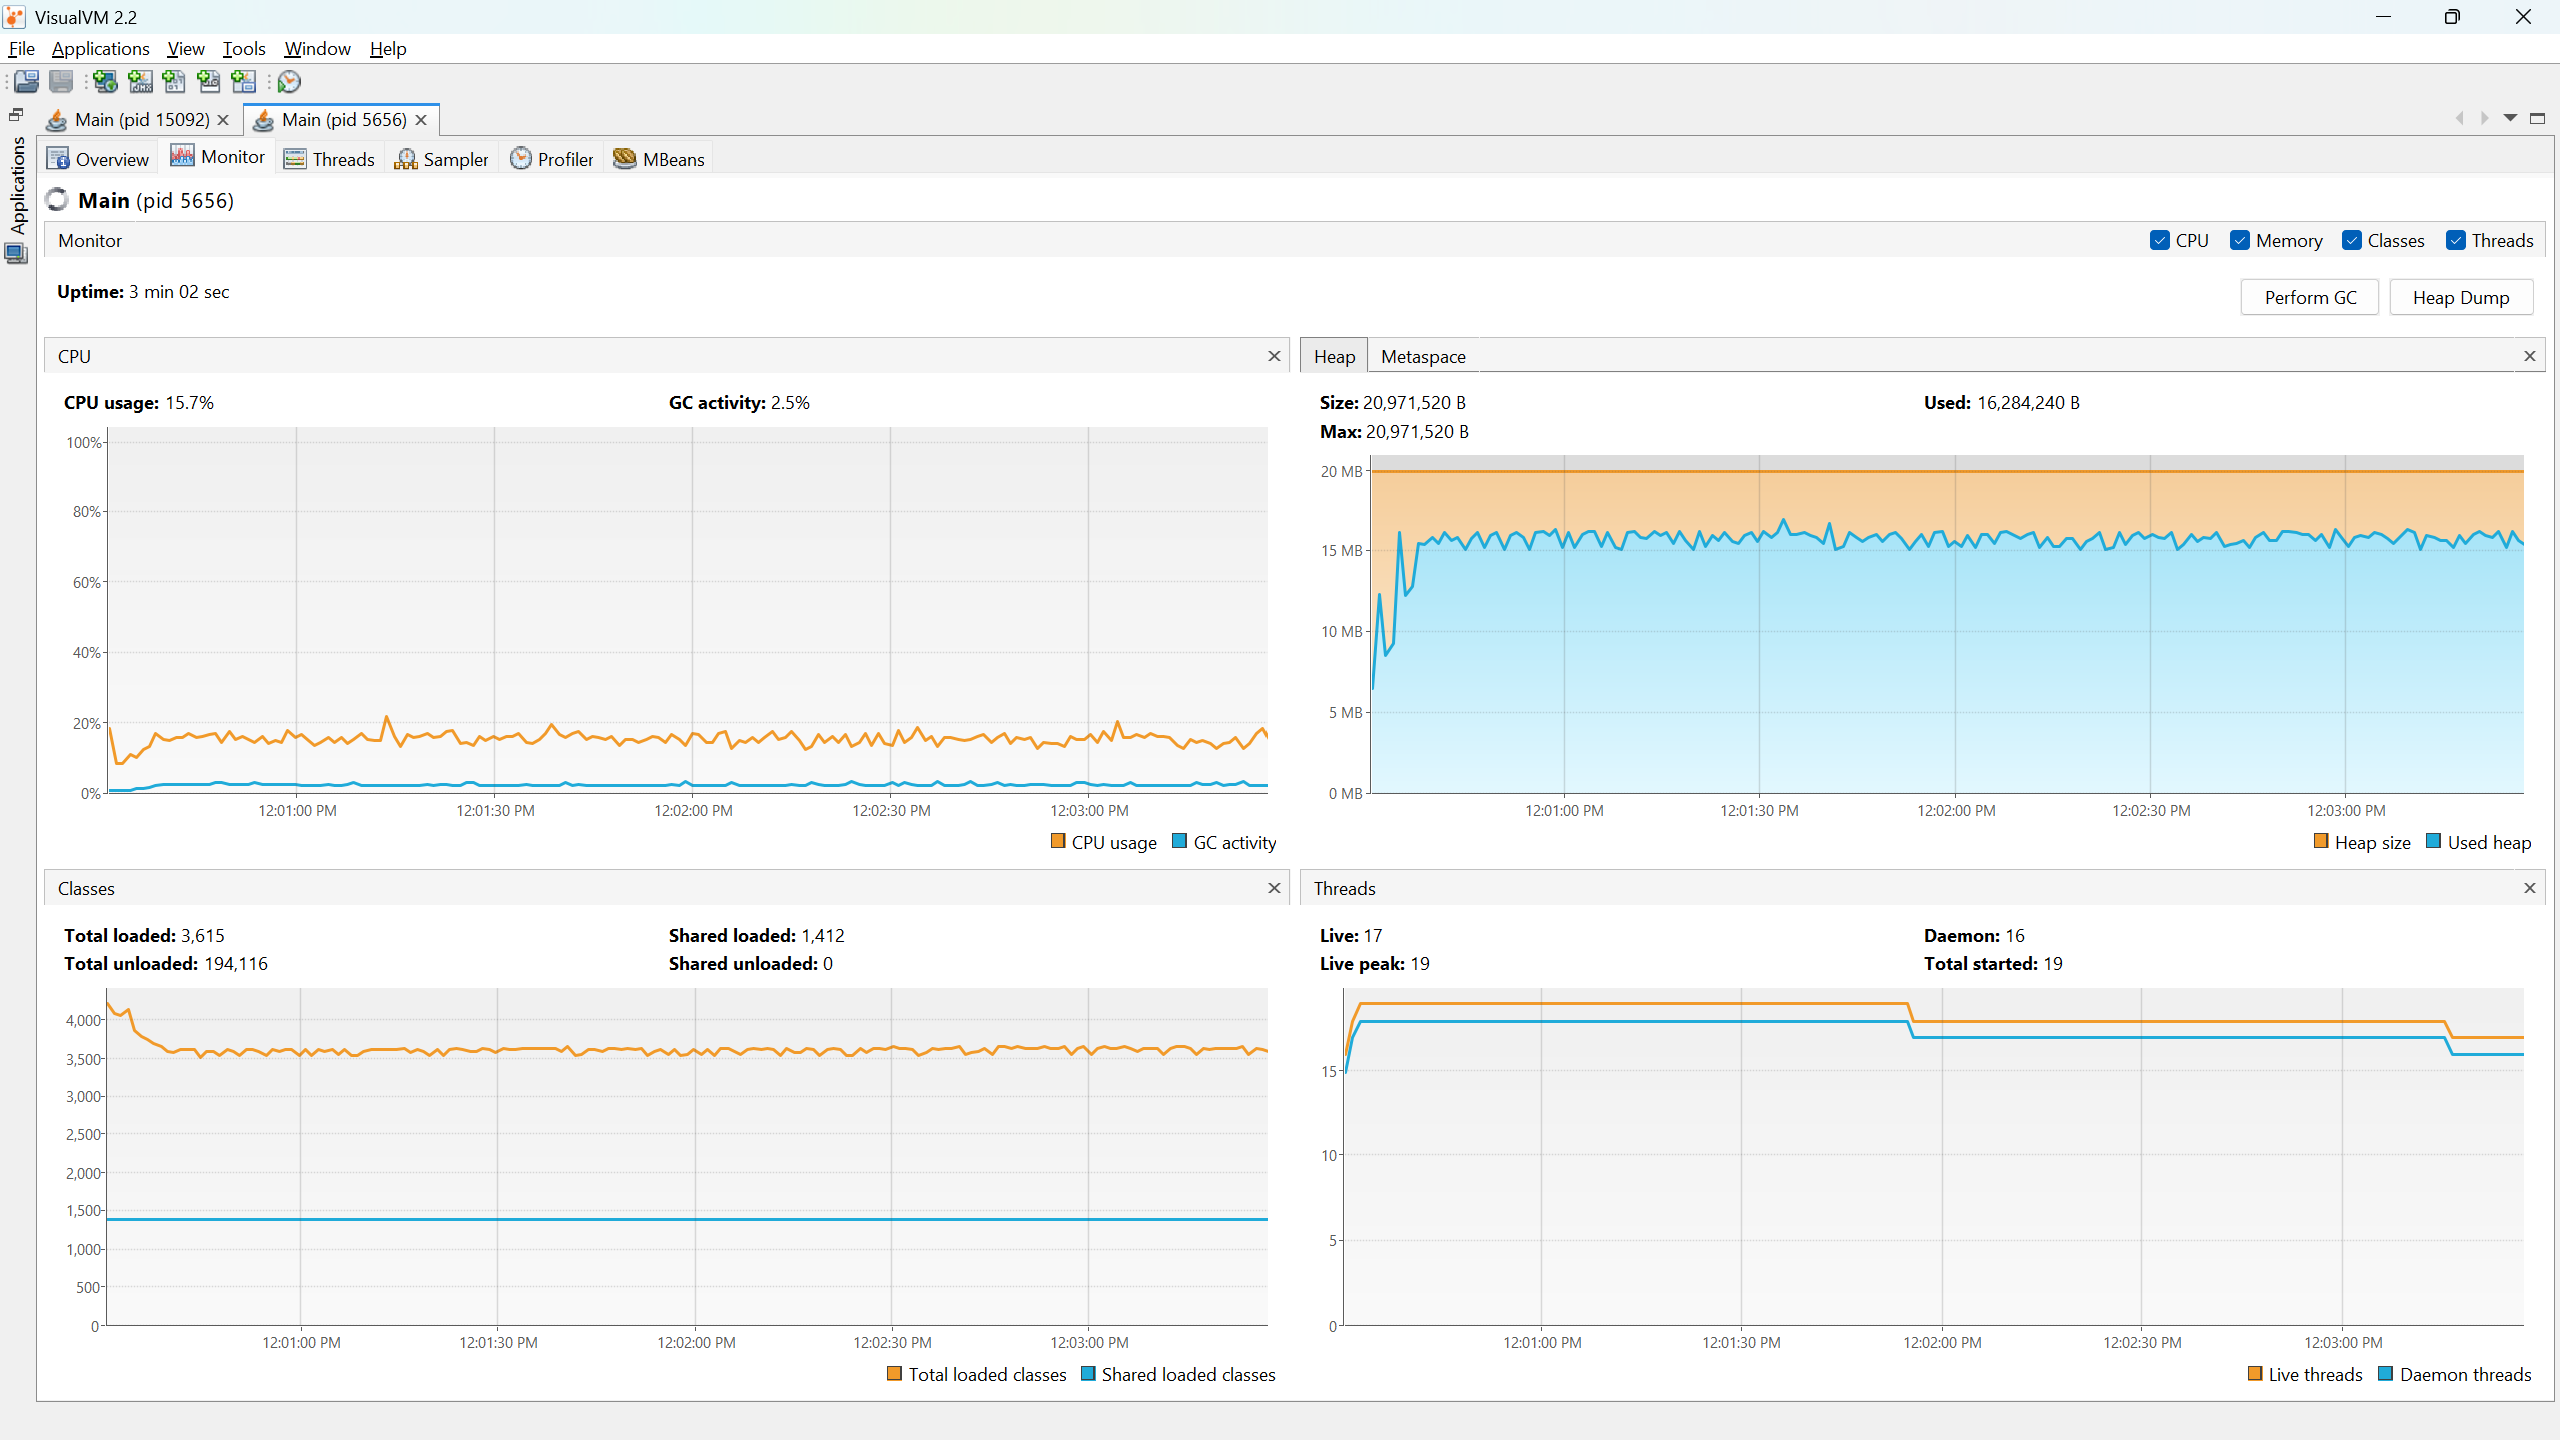
\includegraphics[width=1\linewidth]{visualvm/stable_work}
		\caption{Стабильная работа приложения с ограничением памяти 20 МБ после исправления}
		\label{fig:stablework}
	\end{figure}
	
	Программа стабильно работает через три минуты после запуска(при первом запуске завершилась через 20 секунд)
	
	\newpage
	
	\section{Заключение и выводы}
	
	\textbf{Результаты:}
	\begin{itemize}
		\item Реализованы MBean: \texttt{PointsCounter} (подсчет точек с уведомлениями каждые 10) и \texttt{AverageClickTime} (расчет среднего времени кликов).
		\item Проведен мониторинг в JConsole и профилирование в VisualVM: определена версия Java, построены графики, выявлен класс \texttt{Point} как основной потребитель памяти.
		\item Устранена утечка памяти в \texttt{ArrayList} путем очистки списка.
	\end{itemize}
	
	\textbf{Выводы:}
	\begin{itemize}
		\item MBean созданы, мониторинг и оптимизация проведены.
		\item Процесс поиска утечки памяти задокументирован.
	\end{itemize}
	
	
\end{document}